\documentclass[leqno, openany]{memoir}
\setulmarginsandblock{3.5cm}{3.5cm}{*}
\setlrmarginsandblock{3cm}{3.5cm}{*}
\checkandfixthelayout

\usepackage{amsmath}
\usepackage{amssymb}
\usepackage{amsthm}
%\usepackage{MnSymbol}
\usepackage{bm}
\usepackage{accents}
\usepackage{mathtools}
\usepackage{tikz}
\usetikzlibrary{calc}
\usetikzlibrary{automata,positioning}
\usepackage{tikz-cd}
\usepackage{forest}
\usepackage{braket} 
\usepackage{listings}
\usepackage{mdframed}
\usepackage{verbatim}
\usepackage{physics}
\usepackage{stmaryrd}
\usepackage{mathrsfs} 
\usepackage{ulem} 
\usepackage{stackengine}
%\usepackage{/home/patrickl/homework/macaulay2}

%font
\usepackage[sc]{mathpazo}
\usepackage{eulervm}
\usepackage[scaled=0.86]{berasans}
\usepackage{inconsolata}
\usepackage{microtype}

%CS packages
\usepackage{algorithmicx}
\usepackage{algpseudocode}
\usepackage{algorithm}

% typeset and bib
\usepackage[english]{babel} 
\usepackage[utf8]{inputenc} 
\usepackage[T1]{fontenc}
\usepackage[backend=biber, style=alphabetic]{biblatex}
\usepackage[bookmarks, colorlinks, breaklinks]{hyperref} 
\hypersetup{linkcolor=black,citecolor=black,filecolor=black,urlcolor=blue}

% other formatting packages
\usepackage{float}
\usepackage{booktabs}
\usepackage[shortlabels]{enumitem}
\usepackage{csquotes}
\usepackage{titlesec}
\usepackage{titling}
% \usepackage{fancyhdr}
% \usepackage{lastpage}
\usepackage{parskip}

\usepackage{lipsum}

% delimiters
\DeclarePairedDelimiter{\gen}{\langle}{\rangle}
\DeclarePairedDelimiter{\floor}{\lfloor}{\rfloor}
\DeclarePairedDelimiter{\ceil}{\lceil}{\rceil}


\newtheorem{thm}{Theorem}[section]
\newtheorem{cor}[thm]{Corollary}
\newtheorem{prop}[thm]{Proposition}
\newtheorem{lem}[thm]{Lemma}
\newtheorem{conj}[thm]{Conjecture}
\newtheorem{quest}[thm]{Question}

\theoremstyle{definition}
\newtheorem{defn}[thm]{Definition}
\newtheorem{defns}[thm]{Definitions}
\newtheorem{con}[thm]{Construction}
\newtheorem{exm}[thm]{Example}
\newtheorem{exms}[thm]{Examples}
\newtheorem{notn}[thm]{Notation}
\newtheorem{notns}[thm]{Notations}
\newtheorem{addm}[thm]{Addendum}
\newtheorem{exer}[thm]{Exercise}

\theoremstyle{remark}
\newtheorem{rmk}[thm]{Remark}
\newtheorem{rmks}[thm]{Remarks}
\newtheorem{warn}[thm]{Warning}
\newtheorem{sch}[thm]{Scholium}


% unnumbered theorems
\theoremstyle{plain}
\newtheorem*{thm*}{Theorem}
\newtheorem*{prop*}{Proposition}
\newtheorem*{lem*}{Lemma}
\newtheorem*{cor*}{Corollary}
\newtheorem*{conj*}{Conjecture}

% unnumbered definitions
\theoremstyle{definition}
\newtheorem*{defn*}{Definition}
\newtheorem*{exer*}{Exercise}
\newtheorem*{defns*}{Definitions}
\newtheorem*{con*}{Construction}
\newtheorem*{exm*}{Example}
\newtheorem*{exms*}{Examples}
\newtheorem*{notn*}{Notation}
\newtheorem*{notns*}{Notations}
\newtheorem*{addm*}{Addendum}


\theoremstyle{remark}
\newtheorem*{rmk*}{Remark}

% shortcuts
\newcommand{\Ima}{\mathrm{Im}}
\newcommand{\A}{\mathbb{A}}
\newcommand{\F}{\mathbb{F}}
\newcommand{\G}{\mathbb{G}}
\newcommand{\N}{\mathbb{N}}
\newcommand{\R}{\mathbb{R}}
\newcommand{\C}{\mathbb{C}}
\newcommand{\Z}{\mathbb{Z}}
\newcommand{\Q}{\mathbb{Q}}
\renewcommand{\k}{\Bbbk}
\renewcommand{\L}{\mathbb{L}}
\renewcommand{\P}{\mathbb{P}}
\newcommand{\M}{\overline{M}}
\newcommand{\g}{\mathfrak{g}}
\newcommand{\h}{\mathfrak{h}}
\newcommand{\n}{\mathfrak{n}}
\renewcommand{\b}{\mathfrak{b}}
\newcommand{\ep}{\varepsilon}
\newcommand*{\dt}[1]{%
   \accentset{\mbox{\Huge\bfseries .}}{#1}}
\renewcommand{\abstractname}{Official Description}
\newcommand{\mc}[1]{\mathcal{#1}}
\newcommand{\T}{\mathbb{T}}
\newcommand{\mf}[1]{\mathfrak{#1}}
\newcommand{\mr}[1]{\mathrm{#1}}
\newcommand{\ms}[1]{\mathsf{#1}}
\newcommand{\mt}[1]{\mathtt{#1}}
\newcommand{\on}[1]{\operatorname{#1}}
\newcommand{\ol}[1]{\overline{#1}}
\newcommand{\ul}[1]{\underline{#1}}
\newcommand{\wt}[1]{\widetilde{#1}}
\newcommand{\wh}[1]{\widehat{#1}}
\renewcommand{\div}{\operatorname{div}}
\newcommand{\bir}{\sim_{\mr{bir}}}
\newcommand{\stacks}[1]{\href{https://stacks.math.columbia.edu/tag/#1}{#1}}
\newcommand{\ostar}{\stackMath\mathbin{\stackinset{c}{0ex}{c}{0ex}{\star}{\bigcirc}}}

\DeclareMathOperator{\Der}{Der}
\DeclareMathOperator{\Def}{Def}
\DeclareMathOperator{\Bl}{Bl}
\DeclareMathOperator{\NE}{NE}
\DeclareMathOperator{\Tor}{Tor}
\DeclareMathOperator{\Hom}{Hom}
\DeclareMathOperator{\Ext}{Ext}
\DeclareMathOperator{\End}{End}
\DeclareMathOperator{\ad}{ad}
\DeclareMathOperator{\Aut}{Aut}
\DeclareMathOperator{\Rad}{Rad}
\DeclareMathOperator{\Pic}{Pic}
\DeclareMathOperator{\supp}{supp}
\DeclareMathOperator{\Supp}{Supp}
\DeclareMathOperator{\sgn}{sgn}
\DeclareMathOperator{\spec}{Spec}
\DeclareMathOperator{\Spec}{Spec}
\DeclareMathOperator{\proj}{Proj}
\DeclareMathOperator{\Proj}{Proj}
\DeclareMathOperator{\ord}{ord}
\DeclareMathOperator{\Div}{Div}
\DeclareMathOperator{\depth}{depth}
\DeclareMathOperator{\coker}{coker}

% Section formatting
\titleformat{\section}
    {\Large\sffamily\scshape\bfseries}{\thesection}{1em}{}
\titleformat{\subsection}[runin]
    {\large\sffamily\bfseries}{\thesubsection}{1em}{}
\titleformat{\subsubsection}[runin]{\normalfont\itshape}{\thesubsubsection}{1em}{}

\title{COURSE TITLE}
\author{Lectures by INSTRUCTOR, Notes by NOTETAKER}
\date{SEMESTER}

\newcommand*{\titleSW}
    {\begingroup% Story of Writing
    \raggedleft
    \vspace*{\baselineskip}
    {\Huge\itshape Informal Enumerative Geometry Seminar \\ Spring 2022}\\[\baselineskip]
    {\large\itshape Notes by Patrick Lei}\\[0.2\textheight]
    {\Large Lectures by Various}\par
    \vfill
    {\Large \sffamily Columbia University}
    \vspace*{\baselineskip}
\endgroup}
\pagestyle{simple}

\chapterstyle{ell}


%\renewcommand{\cftchapterpagefont}{}
\renewcommand\cftchapterfont{\sffamily}
\renewcommand\cftsectionfont{\scshape}
\renewcommand*{\cftchapterleader}{}
\renewcommand*{\cftsectionleader}{}
\renewcommand*{\cftsubsectionleader}{}
\renewcommand*{\cftchapterformatpnum}[1]{~\textbullet~#1}
\renewcommand*{\cftsectionformatpnum}[1]{~\textbullet~#1}
\renewcommand*{\cftsubsectionformatpnum}[1]{~\textbullet~#1}
\renewcommand{\cftchapterafterpnum}{\cftparfillskip}
\renewcommand{\cftsectionafterpnum}{\cftparfillskip}
\renewcommand{\cftsubsectionafterpnum}{\cftparfillskip}
\setrmarg{3.55em plus 1fil}
\setsecnumdepth{subsection}
\maxsecnumdepth{subsection}
\settocdepth{subsection}

\begin{document}
    
\begin{titlingpage}
\titleSW
\end{titlingpage}

\thispagestyle{empty}
\section*{Disclaimer}%
\label{sec:disclaimer}

These notes were taken during the seminar using the \texttt{vimtex} package of the editor \texttt{neovim}. 
Any errors are mine and not the speakers'. 
In addition, my notes are picture-free (but will include commutative diagrams) and are a mix of my mathematical style and that of the lecturers.
If you find any errors, please contact me at \texttt{plei@math.columbia.edu}.

\vspace*{1cm}

\noindent\textbf{Seminar Website:}  \url{https://www.math.columbia.edu/~ccliu/Seminars/IEG_S22.html}
\newpage

\tableofcontents

\chapter{Melissa (Feb 03): Virtual fundamental classes in algebraic geometry}%
\label{cha:Melissa_Feb_03_Virtual_fundamental_classes_in_algebraic_geometry}

\section{Overview}
Virtual fundamental classes are well-motivated for us, so we will not motivate them. Let $X$ be a Deligne-Mumford stack, which is \textit{virtually smooth} (which means it has a perfect obstruction theory). A perfect obstruction theory is a class $E = [E^{-1} \to E^0]$ in $D(X)$ which is locally isomorphic to a morphism of vector bundles.

In Li-Tian, the authors consider a \textit{perfect tangent-obstruction complex}
\[ \mc{T}^1 \xrightarrow{o} \mc{T}^2, \]
where $\mc{T}^1$ is the tangent sheaf and $\mc{T}^2$ is the obstruction sheaf. If we consider
\[ 0 \to \mc{T}^1 \to (E^0)^{\vee} \to (E^{-1})^{\vee} \to \mc{T}^2 \to 0, \]
we note that the \textit{virtual tangent bundle} has K-theory class
\begin{align*}
    T^{\mr{vir}} &= \mc{T}^1 - \mc{T}^2 \\
    &= (E^0)^{\vee} - (E^{-1})^{\vee}.
\end{align*}
Thus $E$ has virtual dimension $d \coloneqq \on{rk} E^0 - \on{rk} E^{-1}$, and from the data $(X, E)$, we will produce a \textit{virtual fundamental class} $[X,E]^{\mr{vir}} \in A_d(X, \Q)$. If $X$ is a scheme (for example in Donaldson-Thomas theory), then $[X, E]^{\mr{vir}} \in A_d(X, \Z)$. If $X$ is smooth, then $E = [0 \to \Omega_X]$ and $T^{\mr{vir}} = T_X$. Of course, we should recover the usual fundamental class in this case.

\section{Cones}
Recall the Proj construction from Hartshorne, II.7. Let $X$ be a scheme and $\mc{S}$ be a sheaf of graded $\mc{O}_X$-algebras generated over $\mc{S}_0 = \mc{O}_X$ by a coherent $\mc{S}_1$. Then define $C(\mc{S}) = \Spec (\mc{S}) \to X$, which is an affine scheme over $X$. Because $\on{Sym}^{\bullet} (\mc{S}_1) \twoheadrightarrow \mc{S}$, then $C(\mc{S}) \hookrightarrow C(\on{Sym}^{\bullet} (S_1))$ is a closed embedding.

\begin{exm}
    Consider $X = \Spec k$ and $\mc{S} = k[x,y,z]/(xz-y^2)$. Of corse $\Proj \mc{S}$ is a conic in $\P^2$, and $\Spec \mc{S}$ is $\A^2 / (\pm 1)$, which is a cone. Note that $\on{Sym} \mc{S}_1 = k[x,y,z]$, so $C(\on{Sym}(\mc{S}_1)) = \A^3$.
\end{exm}

Of course, by Hartshorne, Ex. II.5.18, if $\mc{E}$ is locally free, then $\Spec \on{Sym}(E)$ is a vector bundle. The analogous notion for a coherent sheaf $\mc{F}$ is an \textit{abelian cone}. Note that the Stacks Project calls abelian cones vector bundles for some reason.

\section{Local theory on a scheme}
Recall that if $X$ is a smooth manifold, then it has an atlas $U_{\alpha}$ of open sets in $\R^n$. Let $X$ be a scheme. Then $X$ has a cover by affines $U_{\alpha}$, and we have open embeddings $U_{\alpha} = \Spec R_{\alpha} \to X$. Finally, consider a Deligne-Mumford stack $X$. Then we have an \'etale atlas $U_{\alpha} = \Spec R_{\alpha}$. If $X$ is an Artin stack, then replace \'etale with smooth.

Now let $D(X)$ denote the derived category of quasicoherent sheaves of $\mc{O}_X$-modules. Then let $D^{[-1,0]}$ denote the full subcategory on complexes with vanishing cohomology outside of $[-1,0]$ with $h^0$ and $h^1$ coherent.
\begin{defn}
    A \textit{perfect obstruction theory} on $X$ is a complex $E \in D^{[-1,0]}(X)$ with $\phi \colon E \to L_X$, where $L_X$ is the cotangent complex such that $\phi$ induces an isomorphism on $h^0$ and a surjection on $h^{-1}$.
\end{defn}

To understand this, assume that $U$ is an affine scheme with an \'etale morphism to $X$. Then $\phi \colon E \to L_X$ pulls back to $\phi_U \colon E_U \to L_U$. If we consider a closed immersion $i \colon U \hookrightarrow W$ of $U$ into a smooth scheme, we can now do intersection theory a la Fulton. The normal cone $C_{U/W}$ is defined to be
\[ C_{U/W} \coloneqq \Spec \bigoplus_{n \geq 0} \mc{I}^n / \mc{I}^{n+1}. \]
This is a closed subcone of $N_{U/W} = \Spec \on{Sym} \mc{I}/\mc{I}^2$. In this case, we only need to consider the truncated cotangent complex
\[ \tau_{\geq -1} L_U = [\mc{I}/\mc{I}^2] \to i^* \Omega_W. \]
In fact, if $U \to W$ is a local complete intersection, then $\mc{I}/\mc{I}^2$ is locally free and $L_U = [\mc{I}/\mc{I}^2 \to i^* \Omega_W]$. Thus $L_U^{\vee} = [i^* T_W \to \mc{N}_{U/W}]$. If this is surjective, then $U$ is smooth, so we have an exact sequence
\[ 0 \to T_U \to i^* T_W \to \mc{N}_{U/W} \to 0, \]
and therefore $[\mc{I}/\mc{I}^2 \to i^* \Omega_W] = [0 \to \Omega_U] = L_U$. Locally, we have $E_U = [E^{-1} \to E^0]$ a morphism of locally free sheaves, and a morphism $\phi \colon E \to \tau_{\geq -1} L_U$.

\begin{prop}
    Up to quasi-isomorphism, we may assume that $E_U = [E^{-1} \to E^0]$ and $\tau_{\geq -1} L_U = [L^{-1} \to L^0 = E^0]$ with $\phi_0 = \mr{id}$. Given these assumptions, $E^{-1} \to L^{-1}$ is surjective.
\end{prop}

\begin{proof}
    Locally, suppose that $U = \Spec R$. Then let $E^{-1}, E^0, F^{-1}, F^0$ be finitely-generated $R$-modules such that $E^0, F^0$ are free. Then consider $\phi \colon E \to F$. Next, choose a surjection $\pi \colon G \twoheadrightarrow F^{-1}$ with $G$ a finitely-generated free module. Then define
    \[ \wt{E} = [E^{-1} \oplus G \xrightarrow{\mqty(\dd_E & 0 \\ 0 & \mr{id})} E^0 \oplus G], \]
    which is clearly quasi-isomorphic to $E$. Then define $\wt{\phi}$ by $\wt{\phi}_{-1} = \phi^{-1}+ \pi$ and $\wt{\phi}_0 = \phi_0 + \dd_F \circ \pi$. Now $\wt{\phi}_0$ is surjective.

    Next, we may asume that $E = [E^{-1} \to E^0]$ such that $phi_0$ is surjective. We will now replace $F$ by the top row of the cartesian diagram
    \begin{equation*}
    \begin{tikzcd}
        \wt{F}^{-1} \ar{d} \ar{r} & E^0 \ar{d} \\
        F^{-1} \ar{r} & F^0.
    \end{tikzcd}
    \end{equation*}
    Because this is a fiber product, we have a map $E \to \wt{F}$ that is the identity in the $0$-th position.
\end{proof}

Now we return to an \'etale chart $U \to X$, where $X$ is a Deligne-Mumford stack. Applying $\Spec \on{Sym}(-)$ to $E$, we obtain a morphism
\[ E_0 = \Spec \on{Sym}(E^0) \to E_1 = \Spec \on{Sym}(E^{-1}). \]
Then we define 
\[ \underline{\mc{E}} \coloneqq h^1 / h^0 (\check{E}) = [E_1 / E_0], \] 
which is an Artin stack. We also apply this to the \textit{intrinsic normal sheaf}
\[ \underline{\mc{N}}_U \coloneqq h^1 / h^0(( \tau_{\geq -1} L_U )^{\vee}) \cong [\mc{N}_{U/W} / i^* T_W]. \]
Finally, the \textit{intrinsic normal cone} is defined to be
\[ \ul{C}_U \coloneqq [C_{U/W} / i^* T_W], \]
which is a cone stack over $U$. We have a closed embedding 
\[ \ul{C}_U \hookrightarrow \ul{N}_U = [N_{U/W} / i^* T_W] = [C(\mr{Sym}(L^{-1})) / E_0] \]
of $\ul{C}_U$ into an abelian cone stack. Finally, these embed into $\ul{E}_U = [E_1 / E_0]$. Because $C_{U/W}$ has pure dimension $\dim W$, we see that $\ul{C}_U$ has dimension $0$.

\section{Virtual fundamental classes}
We have intrinsic normal cones locally, and fortunately, they glue! Therefore, we have an \textit{intrinsic normal cone} $\ul{C}_X$ which is a cone stack over $X$ of pure dimension $0$, an \textit{intrinsic normal sheaf} $\ul{\mc{N}}_X$ which is an abelian cone stack over $X$, and $\ul{\mc{E}}_X$, which is a vector bundle stack over $X$ smooth of relative dimension $d_1 - d_0 = -d$.

Recall from Fulton that if $E \to X$ is a vector bundle over a scheme of rank $r$, there is a \textit{Gysin map} $0_E^! \colon A_d(E) \to A_{d-r}(X)$. We want to do something similar in the case of a vector bundle stack. In \textit{Cycles groups for Artin stacks}, Kresch gives the following: Let $\mc{E} \to X$ be a vector bundle stack of rank $r$ over a Deligne-Mumford stack. Then there is a Gysin map $0_{\mc{E}}^! \colon A_d(\ul{\mc{E}}) \to A_{d-r}$. Applying this to our situation, the \textit{virtual fundamental class} is given by
\[ [X, E]^{\mr{vir}} \coloneqq 0_{\ul{\mc{E}}_X}^! [\ul{C}] \in A_d(X). \]

\section{Relative version}
Let $X$ be a Deligne-Mumford stack and consider $\pi_{X/M} \colon X \to M$, where $M$ is a smooth Artin stack of pure dimension $m$. If $\pi_{X/M}$ is virtually smooth, then there exists a \textit{relative perfect obstruction theory}
\[ \phi \colon E_{X/M} \to L_{X/M}, \]
where $L_{X/M}$ is the relative cotangent complex. We again require that $\phi$ induces an isomorphism on $h^0$ and a surjection on $h^{-1}$.

If $U$ is an affine scheme with $U \to X$ \'etale, then $U \to M$ is smooth. Also let $i \colon U \hookrightarrow W$ be a closed embedding of $U$ into a smooth scheme and suppose $W \to M$ is smooth of relative domension $d_0$. Then we have the relative intrinsic normal cone
\[ \ul{C}_{U/M} = [C_{U/W} / i^* T_{W/M}] \]
of pure dimension $m$, the relative intrinsic normal sheaf
\[ \ul{\mc{N}}_{U/M} = [\mc{N}_{U/W} / T_{W/M}], \]
and the vector bundle stack $\ul{\mc{E}}_{U/M}$. These also glue nicely, and we obtain
\[ \ul{C}_{X/M} \hookrightarrow \ul{\mc{N}}_{X/M} \hookrightarrow \ul{\mc{E}}_{X/M}, \]
where $\ul{\mc{E}}_{X/M}$ is a vector bundle stack of rank $-d = d_1 - d_0$. Then $[\ul{C}_{X/M}] \in A_m(\ul{\mc{E}}_{X/M})$, and then the \textit{relative virtual fundamental class} is
\[ [X, E_{X/M}]^{\mr{vir}} = 0_{\ul{\mc{E}}_{X/M}}^! [\ul{C}_{X/M}] \in A_{m+d}(X). \]

\chapter{Melissa (Feb 10): Virtual fundamental classes in enumerative geometry}%

Recall our abstract setup of a Deligne-Mumford stack $X$ and a perfect obstruction theory $E$. In this setting, Behrend-Fantechi construct a virtual fundamental class $[X, E]^{\mr{vir}} \in A_d(X)$, where $d$ is the virtual dimension of $X$. There is an equivariant version of this for the action of a reductive group $G$ on a Deligne-Mumford stack $\mc{X}$. Then we will have $L_{\mc{X}} \in D_G(\mc{X})$, so we can consider equivariant perfect obstruction theories $E$. Here, we will have $[\mc{X}, E]^{\mr{vir}} \in A_d^G(\mc{X})$.

For us, we will normally consider $T = (\C^*)^k$. Here, there is a fixed substack $\mc{X}^T$. If we consider
\[ 0 \to \mc{T}^1 \to (E^0)^{\vee} \to (E^{-1})^{\vee} \to \mc{T}^2 \to 0, \]
we know that $\mc{T}^{\mr{vir}} = \mc{T}^1 - \mc{T}^2 = (E^0)^{\vee} - (E^{-1})^{\vee}$. Restricting to the fixed locus, we can decompose the tangent sheaf 
\[ \mc{T}^1_{\mc{X}^T} = \mc{T}^{1,f} \oplus \mc{T}^{1,m} \]
into fixed and moving parts, and similarly for the obstruction sheaf $\mc{T}^2$. Then we have
\[ \mc{T}^{1,f} - \mc{T}^{2,f} = T_{\mc{X}^T}^{\mr{vir}} \]
and the moving part is
\[ \mc{T}^{1,m} - \mc{T}^{2,m} = N^{\mr{vir}}. \]
Graber-Pandharipande proved torus localization for virtual fundamental classes, and in particular, we obtain
\[ [X,E]^{\mr{vir}} = i_* \frac{[\mc{X}^{\C^*}, E^{\C^*}]^{\mr{vir}}}{e_{\C^*}(N^{\mr{vir}})}. \]
Because $A^* (B\C^*) = \Q[t]$, we are considering $[\mc{X}, E]^{\mr{vir}} \in A_d^{\C^*} (\mc{X}) \otimes_{\Q[t]} \Q[t, t^{-1}]$. Note that if $\C^*$ acts trivially on $\mc{Y}$, then $A_d^{\C^*}(\mc{Y}) = A_d(\mc{Y}) \otimes_{\Q} \Q[t]$.

\section{Gromov-Witten theory}

Let $X$ be a smooth projective variety and $\beta \in H_2(X, \Z)$ be an effective curve class. Let $\wt{\mc{X}} = \mc{M}_{g, n}^{\mr{pre}}(X, \beta)$ be the moduli space of genus $g$, $n$-pointed stable maps to $X$ of degree $\beta$. The $\C$-points of this functor are $((C, x_1, \ldots, x_n), f)$, where $C$ is a genus $g$, $n$-pointed prestable curve and $f \colon C \to X$ has $f_* [C] = \beta$.

Taking the locus with finite automorphism groups, we obtain a Deligne-Mumford stack $\mc{X} = \ol{\mc{M}}_{g, n}(X, \beta) \subset \wt{\mc{X}}$, which is an Artin stack. $\mc{X}$ is a proper Deligne-Mumford stack with projective coarse moduli space. Recall that there is a map $\pi_{\wt{\mc{X}}/\mc{M}} \colon \wt{\mc{X}} \to \mc{M}_{g, n}^{\mr{pre}}$, which is a smooth Artin stack of dimension $3g-3 + n$, forgetting the map $f$. We would like to construct a relative perfect obstruction theory.

Consider the diagram
\begin{equation*}
\begin{tikzcd}
    C \ar{d} & C_{\wt{\mc{X}}} \ar{r} \ar{d}{\pi_{\wt{\mc{X}}}} & C_{\mc{M}} \ar{d}{\pi_{\mc{M}}} \\
    \Spec \C \ar{r}{\xi} & \wt{\mc{X}} \ar{r} & \mc{M}
\end{tikzcd}
\end{equation*}
with $f \colon C \to X$. Then we have $h^0(E_{\wt{\mc{X}}/ \mc{M}}^{\vee})_{\xi} = H^0(C, f^* T_X)$ and $h^1(E^{\vee}_{\wt{\mc{X}}/\mc{M}})_{\xi} = H^1(C, f^* T_X)$. Globally, we obtain
\[ h^i(E_{\wt{\mc{X}} / \mc{M}}) = R^i \pi_{\wt{\mc{X}}*}(f_{\mc{X}}^* T_X). \]
Then we obtain 
\[ d_{\wt{\mc{X}}/\mc{M}}^{\mr{vir}} = \chi(C, f^* T_X) = \deg (f^* T_X) + \mr{rk} (f^* T_X)(1-g) = \int_{\beta} c_1(TX) + \dim X (1-g), \]
and therefore we obtain
\[ d_{\wt{\mc{X}}}^{\mr{vir}} = \int_{\beta} c_1(TX) + (\dim X - 3)(1-g) + n. \]
Our stability condition guarantees that any component contracted by $f$ is already stable as a curve. Now let $T$ be a scheme of finite type with a smooth map to $\mc{X}$. Then we have the following diagram:
\begin{equation*}
\begin{tikzcd}
    C_T \ar{d}{\pi_T} \ar{r} & C_{\mc{X}} \ar{d} \\
    T \ar{r} & \mc{X}
\end{tikzcd}
\end{equation*}
with $f_T \colon C_T \to X$. We know that $\pi_T$ is flat and projective over $T$, so define the line bundle
\[ \mc{L} \coloneqq \omega_{\pi_T}(x_1 + \cdots + x_n) \otimes f_T^* \mc{O}_X(3). \]
By the stability condition, $\mc{L}$ is $\pi_T$-ample because $\omega_{\pi_T}(x_1 + \cdots + x_n)$ has degree $2 g_v - 2 + n_v \geq -2$ on any irreducible component $C_v \subset C$. Also, $f_T^* T_X$ is a locally free sheaf on $C_T$, so there exists $N \gg 0$ such that $f_T^* T_X \otimes \mc{L}^N$ is globally generated and $H^1(C_t, f_t^* T_X \otimes \mc{L}_t^N) = 0$. In addition, $\pi_*(\mc{L}^{-N}) = 0$.

Now consider the exact sequence
\[ 0 \to F_t \to (\mc{L}_t^{-N})^{\oplus m} \to f_t^* T_X \to 0 \]
and use the long exact sequence in cohomology, and thus $E^{\vee} \simeq [\mc{T}^1 \xrightarrow{0} \mc{T}^2]$.

\begin{exm}
    Note that $\ol{\mc{M}}_{g, n}(X, 0) = \ol{\mc{M}}_{g,n} \times X$. Here, given $((C, z_1, \ldots, z_n) f)$, we must have $f(C) = x$, for some $x \in X$. Then $H^i(C, f^* T_X) = H^i(C, \mc{O}_C) \otimes T_x X$, and so we obtain
    \[ E_{\mc{X}/\mc{M}} = pr_2^* \Omega_X \otimes pr_1^* E^{\vee} \xrightarrow{0} pr_2^* \Omega_X. \]
    Note that $L_{\mc{X}/\mc{M}} = [0 \to pr_2^* \Omega_X$. Thus $\mc{T}^1 = \mc{T}_{\mc{X}}$ and $\mc{T}^2 = pr_2^* T_X \otimes pr_1^* E^{\vee}$, where $E = (\pi_{\mc{M}})_* \omega_{\pi_{\mc{M}}}$. Finally, we see that
    \[ [\mc{M}_{g, n}(X, 0)]^{\mr{vir}} = e(\mr{Ob}) \cap [\ol{M}_{g, n}] \in A_{(\dim X - 3)(1-g) + n}. \]
\end{exm}

\section{Remarks on equivariant localization}
Let $G = \C^*$ act on a stack $\mc{X}$. Then to do localization, we need to check that
\begin{enumerate}
    \item There exists a $G$-equivariant embedding $\mc{X} \hookrightarrow \mc{Y}$ of $\mc{X}$ into a smooth Deligne-Mumford stack.
    \item There exists a global locally free resolution $E = [E^{-1} \to E^{-2}]$.
\end{enumerate}
Thus doing equivariant enumerative geometry required constructing a $G$-equivariant embedding of $\mc{X}$ into a smooth stack. Then a result of Chang-Kiem-Li in 2017 allows us to remove the first condition and weaken the second (we only nneed a global resolution on the fixed locus).

\chapter{Song (Feb 17): Crepant transformation conjecture for toric Deligne-Mumford stacks, part 1}%

The crepant transformation conjecture roughly says:
\begin{conj}[Ruan, etc]
    For a pair of $K$-equivalent manifolds/orbifolds/Deligne-Mumford stacks $X_{\pm}$, their quantum cohomology/Gromov-Witten theory should be related.
\end{conj}

Here, by \textit{K-equivalent} we mean (following C-L Wang) that there exists a diagram
\begin{equation*}
\begin{tikzcd}
    & \wt{X} \ar{dl}{f_+} \ar{dr}{f_-} \\
    X_+ \ar[dashrightarrow]{rr}{\varphi} & & X_-
\end{tikzcd}
\end{equation*}
where $\varphi$ is birational, $f_{\pm}$ are projective and birational, and $f_+^* K_{X_+} = f_-^* K_{X_-}$. Coates-Iritani-Jiang formulated and proved the crepant transformation conjecture for toric Deligne-Mumford stacks and complete intersections.

\section{Toric geometry}
Note that toric crepant transformations correspond to wall-crossings of GIT stability conditions. There are three types of this.

\begin{exm}[Crepant (partial) resolution]
    Here, we have a morphism $X_+ \to \abs{X_-}$ that partially resolves singularities of $X_-$. In our example, we will consider $X_+ = K_{\P^2} \dashrightarrow [\C^3 / \mu_3] = X_-$. Then the toric fan of $K_{\P^2}$ is generated by $b_1 = (1,0,1), b_2 = (0,1,1), b_3 = (-1,-1,1), b_4 = (0,0,1)$. The toric fan of $[\C^3 / \mu_3]$ is generated by $b_1, b_2, b_3$, and there is a singularity at $b_4$, so to get $K_{\P^2}$ we subdivide the triangle.

    The GIT data for $K_{\P^2}$ is given by $0 \to L \to \Z^4 \xrightarrow{(b_1, b_2, b_3, b_4)} \Z^3 \to 0$. Dualizing, we have a surjection $(\Z^4)^{\vee} \xrightarrow{(1,1,1,-3)} L^{\vee} \to 0$. In $L_{\R}^{\vee}$, we see that there is a positive chamber and a negative chamber, and in the positive chamber we obtain $K_{\P^2}$ and in the negative chamber we obtain $[\C^3 / \mu_3]$.
\end{exm}

\begin{exm}[Flop]
    Consider $X_{\pm} = \mc{O}_{\P^1}(-1) \oplus \mc{O}_{\P^1}(-1)$. These are related by an Atiyah flop. The flop corresponds to exchanging the two diagonals of a square. In this case, we still have a $1$-dimensional secondary fan with two chambers.
\end{exm}

\begin{exm}[Gerbe flop]
    Consider $X_+ = \P(2,2)$ and $X_- = \P^1 \times B\mu_2$. Note that both rigidified stacks are isomorphic to $\P^1$. The GIT data is given by $\Z^3 \to \Z \times \Z_2 \to 0$, where $b_1 =(1,1), b_2 = (-1,1), b_3 = (1,0)$. If we choose $b_1, b_2$ we obtain $X_-$ and if we choose $b_2, b_3$ we obtain $X_+$. The secondary fan has $D_1 = (1,0), D_2 = (1,2), D_3 = (0,2)$, where the bottom chamber corresponds to $X_+$ and the top chamber corresponds to $X_-$.
\end{exm}

Returning to the crepant resolution, we can tensor the lattice data to obtain
\[ 0 \to \C^* \to (\C^*)^4 \to (\C^*)^3 \to 0. \]
We will let $Q \coloneqq (\C^*)^3$ be the dense open torus in $X_{\pm}$. Thus $T \coloneqq (\C^*)^4$ also acts on $X_{\pm}$. We will work $T$-equivariantly.

Now note that $IX_- = X_- \sqcup B \mu_3 \sqcup B \mu_3$. The two copies of $B \mu_3$ are called the \textit{twisted sectors} and will be labeled by $\frac{1}{3}, \frac{2}{3}$. The untwisted sector will be labeled by $0$. Then we take Chen\footnote{A UMass professor!}-Ruan cohomology and obtain
\[ H^*_{CR}(X_-) = \Q \mathbb{1} \oplus \Q \mathbb{1}_{\frac{1}{3}} \oplus \Q \mathbb{1}_{\frac{2}{3}}, \]
where the twisted sectors live in degrees $2, 4$ respectively. On the other hand, $X_+$ is a scheme, so $I_{X_+} = X_+$ and
\[ H^*(X_+) = \Q \mathbb{1} \oplus \Q H \oplus \Q H^2. \]
Note that $L^{\vee}_{\Q} \cong H^2_{CR}(X_{\pm})$. We will call its rank $r$. We can also define $T, Q$-equivaraint versions of everything and there exists a $T$-equivariant orbifold Poincar\'e pairing
\[ (\alpha, \beta) \coloneqq \int_{IX} \alpha \cup \on{inv}^* \beta. \]
Here, $\on{inv} \colon IX \to IX$ takes an automorphism to its inverse.

\section{Quantum cohomology/Gromov-Witten theory}
First, we will define ($T$-equivariant) Gromov-Witten invariants. Choose $g, n \in \Z_{\geq 0}$, $d \in H_2(\abs{X}, \Z)$, $\alpha_1, \ldots, \alpha_n \in H^*_{CR, T}(X)$, and $k_1, \ldots, k_n \in \Z_{\geq 0}$ defining the descendent insertions. Then we define
\[ \ev{\tau_{k_1}(\alpha_1) \cdots \tau_{k_n}(\alpha_n)}^X_{g,n,d} = \int_{[X_{g,n,d}]^{\mr{vir}}} \prod (\on{ev}_i^* \alpha_i) \psi_i^{k_i}. \]
Note that the moduli spaces are not compact, so we need to use $T$-equivariant localization. 

With the Gromov-Witten invariants, we can now define the quantum product. Let $\phi_0 = 1$, $\phi_1, \ldots,\phi_r$ be a basis for $H^2$, and $\phi_{r+1}, \ldots, \phi_N$ be the completion to a homogeneous basis for $H^*$. Let $\tau^0, \ldots, \tau^N$ be the corresponding coordinates. For $\tau = \sum \tau^i \phi_i$, define
\[ (\phi_i *_{\tau} \phi_j, \phi_k) = \sum_{d \geq 0} \sum_{n \geq 0} \frac{1}{n!} \ev{\phi_i, \phi_j, \phi_k, \tau, \ldots, \tau}_{0,n+3, d}^X. \]
This is a commutative and associative product which has a nonequivariant limit. The reason for this is because the evaluation maps are proper (a consequence of $X$ being semiprojective).

The next thing to define are the $J$-functions. Again write $\tau = \sum_{i=1}^r \tau^i \phi_i$. Then define the \textit{$J$-function}
\[ J_T^X(\tau, z) = 1 + \sum_{d \geq 0} \sum_{n \geq 0} \sum_{i=0}^N \frac{1}{n!} \ev{1, \tau^n, \frac{\phi_i}{z - \psi_{n+2}}}_{0, n+2, d}^X \phi^i. \]
By a result of Givental and Coates-Corti-Iritani-Tseng, there is a mirror theorem stating that
\[ J_T^X(\tau, z) = I_T^X(y, z) \]
under the mirror map $\tau = \tau(y)$. The $I$-function is an explicit hypergeometric function (here, we need $X$ weak Fano).

We will now discuss $I$-functions and the extended complex moduli for the example of the crepant resolution. Let $\lambda_1, \ldots, \lambda_4 \in H_T^2(\mr{pt})$ be the $T$-equivariant parameters. Then set 
\[R_T = H_T^*(\mr{pt}, \C) = \C[\lambda_1, \ldots, \lambda_4]. \]
Continuing, let $u_1^{\pm}, \ldots, u_4^{\pm} \in H^2_{CR, T}(X_{\pm})$ be the $T$-equivariant Poincar\'e duals of the ``divisors'' corresponding to the $b_i$. Also define
\[ \sigma_+ = H \log y_+ + \lambda_1 + \cdots + \lambda_4, \qquad \sigma_i = -\lambda_4 \log y_i + \lambda_1 + \cdots + \lambda_4. \]
Now we may define the $I$-functions of $X_{\pm}$ by
\begin{align*}
    I_+(y_+, z) &= z \cdot e^{\frac{\sigma_+}{z}} \sum_{d \in \Z} y_+^d \prod_{j=1}^4 \frac{\Gamma\qty(1+\frac{u_j^+}{z})}{\Gamma\qty(1 + \frac{u_j^+}{z} + D_j \cdot d)} \cdot \mathbb{1} \\
    I_-(y_-, z) &= z \cdot e^{\frac{\sigma_-}{z}} \sum_{d \in \frac{1}{3}\Z} y_-^{-3d} \cdot \prod_{j=1}^4 \frac{\Gamma\qty(1-\ev{-D_j \cdot d} + \frac{u_j^-}{z})}{\Gamma\qty(1 + \frac{u_j^-}{z}+D_j \cdot d)}  \mathbb{1}_{\ev{-d}},
\end{align*}
where $\ev{d}$ denotes the fractional part of $d$. The $I$-functions have some nice properties. For example, $I_{\pm}(y_{\pm}, z)$ are locally analytic near the ``large radius limit point'' $P_{\pm}$ of $X_{\pm}$ in the extended complex moduli space, which in our case is just the secondary variety corresponding to the secondary fan, which is simply $\P(1,3)$. The point $P_+$ is a smooth point and $P_-$ is an orbifold point. Thus we can relate $y_+ = y_-^{-3}$. Based on this oversimplified picture, we can state the following result:

\begin{thm}[Crepant transformation conjecture, oversimplified]
    There exists a degree-preserving $R_T$-linear isomorphism $\mathbb{U} \colon H^*_{CR, T}(X_-, \C) \to H^*_{CR, T}(X_+, \C)$ such that $I_+(y_+, z) = \mathbb{U} I_-(y_-, z)$ after analytic continuation.
\end{thm}

\chapter{Song (Feb 24): Crepant transformation conjecture for toric Deligne-Mumford stacks, part 2}%

Recall the oversimplified statement of the crepant transformation conjecture discussed previously:
\begin{thm*}
    There exists a degree-preserving $R_T$-linear isomorphism $\mathbb{U} \colon H^*_{CR, T}(X_-, \C) \to H^*_{CR, T}(X_+, \C)$ such that $I_+(y_+, z) = \mathbb{U} I_-(y_-, z)$ after analytic continuation.
\end{thm*}

\section{Technical discussion of the simplified result}

Begin by recalling the $I$-functions corresponding to $X_+ = K_{\P^2}$ and $X_- = [\C^3 / \mu_3]$. We should note here that in this case, $u_4^- = 0$ and $u_1^+ u_2^+ u_3^+ = 0$. We will reproduce the $I$-functions below:
\begin{align*}
    I_+(y_+, z) &= z \cdot e^{\frac{\sigma_+}{z}} \sum_{d \in \Z} y_+^d \prod_{j=1}^4 \frac{\Gamma\qty(1+\frac{u_j^+}{z})}{\Gamma\qty(1 + \frac{u_j^+}{z} + D_j \cdot d)} \cdot \mathbb{1} \\
    I_-(y_-, z) &= z \cdot e^{\frac{\sigma_-}{z}} \sum_{d \in \frac{1}{3}\Z} y_-^{-3d} \cdot \prod_{j=1}^4 \frac{\Gamma\qty(1-\ev{-D_j \cdot d} + \frac{u_j^-}{z})}{\Gamma\qty(1 + \frac{u_j^-}{z}+D_j \cdot d)}  \mathbb{1}_{\ev{-d}},
\end{align*}

The main tool here that we will use is the Mellin-Barnes analytic continuation. This is a classical tool for analytic continuation of hypergeometric functions. Replacing $z = 2 \pi i$, consider the functions
\begin{align*}
    H_+(y_+) &= e^{\frac{\sigma_+}{2 \pi i}} \sum_{d \in \Z} y_+^d \prod_{j=1}^4 \frac{1}{\Gamma\qty(1 + \frac{u_j^+}{2 \pi i} + D_j \cdot d)} \cdot \mathbb{1} \\
    H_-(y_-, z) &= e^{\frac{\sigma_-}{2 \pi i}} \sum_{d \in \frac{1}{3}\Z} y_-^{-3d} \cdot \prod_{j=1}^4 \frac{1}{\Gamma\qty(1 + \frac{u_j^-}{2 \pi i}+D_j \cdot d)}  \mathbb{1}_{\ev{d}},
\end{align*}
This allows us to define the $T$-equivariant \textit{gamma classes} of $X_{\pm}$ by
\begin{align*}
    \wh{\Gamma}_{X_+} &= \prod_{j=1}^4 \Gamma(1 + u_j^+), \\
    \wh{\Gamma}_{X_-} &= \sum_{f = 0,\frac{1}{3}, \frac{2}{3}} \prod_{j=1}^4 \Gamma(1 - \ev{D_j \cdot f} + u_j^-) \mathbb{1}_f.
\end{align*}
We can relate $I$ and $H$ by $I \approx \wh{\Gamma} \smile \on{inv}^* H$. Now we will work with the $H$-functions, and we will consider analytic continuation of $H_{\pm}$ under the fixed-point basis. At the point $p_1$, we have $u_1^+ |_{p_1} = 0$, so we have
\begin{align*}
    H_+(y_+) |_{p_1} &= e^{\frac{\sigma_1 |_{p_1}}{2 \pi i}} \sum_{d \in \Z_{\geq 0}} \frac{y_+^d}{\Gamma(1+d)} \cdot \frac{1}{\Gamma\qty(1 + \frac{u_2^+ |_{p_1}}{2\pi i} + d)\Gamma\qty(1 + \frac{u_3^+ |_{p_1}}{2\pi i} + d)\Gamma\qty(1 + \frac{u_4^+ |_{p_1}}{2\pi i} - 3d)} \\
    &= e^{\frac{\sigma_1 |_{p_1}}{2 \pi i}} \sum_{d \in \Z_{\geq 0}} y_+^d {(-1)}^{-3d} \frac{\sin\qty(-\pi \frac{u_4^+|_{p_1}}{2 \pi i}) \Gamma\qty(-\frac{u_4^+|_{p_1}}{2\pi i} + 3d)}{\pi\cdot  \Gamma(1+d) \Gamma\qty(1+\frac{u_2^+|_{p_1}}{2\pi i}+d)\Gamma\qty(1+\frac{u_3^+|_{p_1}}{2\pi i}+d)} \\
    &= e^{\frac{\sigma_1 |_{p_1}}{2 \pi i}} \sum_{d \in \Z_{\geq 0}} \on{Res}_{s=d} \frac{\Gamma(s) \Gamma(1-s) e^{-2\pi i s} y_+^s\sin\qty(-\pi \frac{u_4^+|_{p_1}}{2 \pi i}) \Gamma\qty(-\frac{u_4^+|_{p_1}}{2\pi i} + 3s)}{\pi\cdot  \Gamma(1+s) \Gamma\qty(1+\frac{u_2^+|_{p_1}}{2\pi i}+s)\Gamma\qty(1+\frac{u_3^+|_{p_1}}{2\pi i}+s)} \dd{s}
\end{align*}
because $\Gamma(x)$ has simple poles at $x \in \Z_{\leq 0}$ and $\Gamma(x) \Gamma(1-x) = \frac{\pi}{\sin(\pi x)}$. Call the complicated function in the final expression $F(s)$. This has poles at all integers and at $\frac{1}{3} \frac{u_4^+|_{p_1}}{2 \pi i} - \frac{1}{3} \Z_{\geq 0}$. But now if $C$ is a contour, we obtain the integral
\[ e^{\frac{\sigma_+ |_{p_1}}{2 \pi i}} \int_C F(s) \dd{s}. \]
Therefore $H_+(y_+) |_{p_1}$ is a sum of residues at poles to the right of $C$, which is the integral for $\abs{y_+}$ small. Taking the analytic continuation from right to left, we obtain the same integral for $\abs{y_+}$ large, which is the same as small $\abs{y_-}$. But now $H_+(y_+) |_{p_1}$ is a sum of residues at poles to the left of $C$. Omitting the explicit computations, we obtain
\[ H_+(y_+)|_{p_1} = C_0 H_-(y_-)|_{(p_4, 0)} + C_{\frac{1}{3}} H_-(y_-)|_{\qty(p_4, \frac{1}{3})} + C_{\frac{2}{3}} H_-(y_-)|_{\qty(p_4, \frac{2}{3})}. \]
After more explicit computations, we obtain the desired result.

For general $X_{\pm}$, suppose we have a $3$-dimensional cone with chambers $\pm$ with a wall. Set $\mc{M}$ to be approximately the toric variety defined by the two chambers. Then $\mc{M}$ is the total space of a vector bundle on the curve $\mc{C} = \P(a,b)$ corresponding to the wall. On $\mc{C}$, there are points $p_+, p_-$ coresponding to the respective large radius limits. We have analytic problems, so we will consider the formal neighborhhood of $\mc{C}$ in $\mc{M}$. Once we do this, we can apply the Mellin-Barnes method.

\section{Fourier-Mukai transform}

Recall that we have the diagram
\begin{equation*}
\begin{tikzcd}
    & \wt{X} \ar{dl}{f_+} \ar{dr}{f_+} \\
    X_+ \ar[dashrightarrow]{rr} & & X_-.
\end{tikzcd}
\end{equation*}
Because this diagram is a $K$-equivalence, we have a \textit{Fourier-Mukai transform}
\[ FM \colon K_T^0(X_-) \xrightarrow{\sim} K_T(X_+) \qquad E \mapsto (f_+)_+ (f_-)^* E. \]
\begin{thm}
    There exists a commutative diagram
    \begin{equation*}
    \begin{tikzcd}
        K_T^0(X_-) \ar{r}{FM} \ar{d}{\Psi_-} & K_T^0(X_+) \ar{d}{\Psi_+} \\
        H^*_{CR,T}(X_-) \ar{r}{\mathbb{U}} & H_{CR,T}(X_+).
    \end{tikzcd}
    \end{equation*}
    The $\Psi_{\pm}$ are related to the ``$\wt{\Gamma}$-integral structure'' where roughly we have
    \[ \Psi(E) \approx \wt{\Gamma}_X \cup \on{inv}^* \wt{\on{ch}}(E). \]
\end{thm}
This result is proved by explicit computation. But now because the Fourier-Mukai transform has a non-equivariant limit, so does $\mathbb{U}$.

\section{Related work}

First, there is some related work in physics by Hori-Romo. In this, the Mellin-Barnes analytic continuation of the hemisphere partition function (the contour integral) corresponds to transportation of branes (the Fourier-Mukai transform).

Second, there is the work of Borisov-Horja. They replace our diagram by the diagram
\begin{equation*}
\begin{tikzcd}
    K^0(X_-) \ar{r}{FM} \ar{d}{MS_-} & K^0(X_+) \ar{d}{MS_+} \\
    (\on{Sol}(U_-))^{\vee} \ar{r} & (\on{Sol}(U_+))^{\vee},
\end{tikzcd}
\end{equation*}
where the bottom row consists of solutions spaces to hypergeometric systems. The bottom arrow is also a Mellin-Barnes integral, and the vertical arrows are so-called ``mirror symmetry'' maps. CIJ is a generalization of this.

Third, there is the work of Gonzalez-Woodward. They have a wall-crossing formula for genus-0 Gromov-Witten theory for general variation of GIT stability condition, which is a generalization of CIJ.

Finally, we can upgrade the simplified version by replacing orbifold cohomology by Givental's loop spaces. There are other statements of the crepant transformation conjecture in quantum cohomology, but some of them have well-definedness issues. Unfortunately, we do not have the time to discuss these.

\chapter{Che (Mar 03): Quantum groups and quantum cohomology, part 1}%

\section{Nakajima quiver varieties}

Let $Q$ be a quiver with set of vertices $I$. Then let $\ol{Q}$ be the framed double of $Q$. Choose dimension vectors $v, w \in \Z^I$. Then let $V_i = \C^{v_i}, W_i = \C^{w_i}$. Then define $\ms{Rep}_{\ol{Q}}$ to be the sum of
\[ \bigoplus_{i, j \in I} \Hom(V_i, V_i)^{\oplus q_{ij}} \oplus \bigoplus_{i \in I} \Hom(V_i, W_i) \]
and its dual. This has an action of $\prod GL(V_i)$ which preserves the symplectic form, so we have a moment map $\mu$. Then we define
\[ \mc{M}_{\theta}^Q(v, w) = \ms{Rep}_{\ol{Q}} \sslash \sslash_{\theta} \prod GL(V_i) = \mu^{-1}(0) \sslash_{\theta} \prod GL(V_i). \]

\begin{exm}
    Let $Q$ be the trivial quiver with one vertex. Then $\mc{M}^Q(k, n) = T^* Gr(k, n)$.
\end{exm}

\begin{exm}
    If $Q$ is the quiver with one vertex and one loop, then $\mc{M}^Q(n, 1) = \mr{Hilb}(\C^2, n)$.
\end{exm}

Nakajima quiver varieties have various group actions. First, define
\[ G_w \coloneqq \prod_{i \in I} GL(W_i). \]
Then we may define
\[ G_{\mr{edge}} \coloneqq \prod_{i \neq j \in I} GL(q_{ij}) \times \prod_{i \in I} Sp(2 q_{ii}) \times \C_{\hslash}^{\times}. \]
Here, the $\C^{\times}_{\hslash}$ scales the symplectic form with weight $\hslash$. Now let $A \subset G_W$ be the maximal torus. 

\begin{exm}
    Consider $T^* Gr(k, n)$. Then $A = (\C^{\times})^n$, and we have
    \[ (T^* Gr(k, n))^A = \qty{\ev{e_{i_1}, \ldots, e_{i_k}} \mid \qty{i_1, \ldots, i_k} \subset [n]} = \binom{[n]}{k}. \]
    Now define $X(n) \coloneqq \bigsqcup_k T^* Gr(k, n)$. Clearly we have $X(n)^A = \mc{P}(n)$. Noting that $X(1) = \mr{pt} \sqcup \mr{pt}$ and $X(2) = \mr{pt} \sqcup T^* \P^1 \sqcup \mr{pt}$, we in fact have
    \[ X(n)^A = \underbrace{X(1) \times \cdots \times X(1)}_{n\text{ times}}. \]
\end{exm}

In general, define $\mc{M}^Q(w) \coloneqq \bigsqcup_v \mc{M}^q(v, w)$. Then we have
\[ (\mc{M}^Q(w))^A = \prod_{i \in I} (\mc{M}^Q(\delta_i))^{w_i}. \]
Now consider $\C^{\times} \hookrightarrow A$, where $z \mapsto (\underbrace{z, \ldots, z}_m, \underbrace{1, \ldots, 1}_{n-m})$. Then in fact $(X(n))^{\C^{\times}} = X(m) \times X(n-m)$.

We also note that $(\mu^{-1}(0) \times V_i) \sslash_{\theta} \prod GL(V_i)$ is a vector bundle $\mc{V}_i$ on $\mc{M}^!(v, w)$. The Chern classes of these $\mc{V}_i$ are called \textit{tautological classes}.

\section{Quantum cohomology}

Let $X$ be a smooth variety with the action of a reductive group $G$ with $X^G$ compact. Define the quantum product by
\[ (\gamma_1 * \gamma_2, \gamma_3) = \sum_{\beta \in H_2(X)_{\mr{eff}}} q^{\beta} \ev{\gamma_1, \gamma_@, \gamma_3}_{0,3,\beta}. \]
Here, $\gamma_i \in H_G^*(X)$ and $(\gamma_1, \gamma_2) = \int_X \gamma_1 \cup \gamma_2$. Our goal is to describe this quantum cohomology in terms of the action of a quantum group. This connection seems surprising, but there is some previous literature on this.

\begin{itemize}
    \item In 1994, Nakajima constructed an action of $\mc{U}(\mf{g})$ on $H^{\bullet}(\mc{M}^Q(w))$, where $Q$ is the quiver with adjacency matrix given by the Cartan matrix of $\mf{g}$.
    \item Nekrasov-Shatashvili proved a correspondence between 2D $N=2$ supersymmetric gauge theories and so-called Heisenberg spin chains. Usually, there is a quantum group action on the Heisenberg spin chains producing operators commuting with the Hamiltonian.
    \item Maulik-Okounkov identified $(H_G^*(X), *)$ with a subalgebra of a quantum group called the Yangian.
\end{itemize}

\section{Stable envelopes}

First, we will construct the stable envelope. This will give us an $R$-matrix, which will in turn give us the Yangian.

Consider the action of $A$ on $X = \mc{M}^Q(v, w)$. Fix a pair of tori $A \subset T \subset G_w \times G_{\mr{edge}}$ where $A$ preserves the symplectic form. Consider all of the $A$-weights of $\mc{N}_{X^A/X}$. These partition the Lie algebra $\mf{a} = \mr{cochar}(A) \otimes_{\Z} \R$ (the Lie algebra of the maximal compact) into chambers.

\begin{exm}
    Consider $T^* \P^{n-1}$. Then the weights are $a_i - a_j$, which are exactly the roots of $SL_n$.
\end{exm}

\begin{defn}
    Let $C$ be a chamber of $\mf{a}$ and let $Y \in \pi_0(X^A)$. Then the \textit{attracting set} of $Y$ with chamber $C$ is defined to be
    \[ \mr{Attr}_C(Y) \coloneqq \qty{x \in X \mid \lim_C(x) \in Y}. \]
    Here, $\lim_C(x) = \lim_{z \to 0} \sigma(z)$ for all $\sigma \in C$. Now we may define
    \[ \mr{Attr}_C^f(Y) = \bigcup_{Y' < Y} \mr{Attr}_C(Y'), \]
    where $Y' < Y$ if $Y' \cap \ol{\mr{Attr}_C(Y)} \neq \emptyset$.
\end{defn}

\begin{exm}
    In the example of $T^* \P^1$, let $u = a_1 - a_2$. Then at $0$, we have weight $-u-\hslash$ in the fiber direction and $u$ in the base direction and at $\infty$ we have weight $-u$ in the base direction and $u-\hslash$ in the fiber direction. Then choose $C = \qty{u > 0}$. Note $X^A = 0 \sqcup \infty$. We then have $\mr{Attr}_C(0) = \P^1 \setminus \infty$ and $\mr{Attr}_C(\infty) = F_{\infty}$. We also have $\mr{Attr}_C^f(0) = \P^1 \cup F_{\infty}$ and $\mr{Attr}_C^f(\infty) = F_{\infty}$.
\end{exm}

\begin{defn}
    A \textit{polarization} is a choice of $T^{1/2} \in K_T(X)$ such that $T_X = T^{1/2} \oplus \hslash^{-1} (T^{1/2})^{\vee}$.
\end{defn}

\begin{exm}
    For $T^* \P^1$, let $T^{1/2} = \pi^*(\Omega_{\P^1})$.
\end{exm}

Next, we will define a degree in $A$. Consider
\[ H_T^*(X^A) = H^*_{T/A}(X^A) \otimes_{\C[\mf{t}/\mf{a}]} \C[\mf{t}], \]
where $\mf{a} = \ms{Lie}(A)$ and $\mf{t} = \ms{Lie}(T)$. Note that $\C[\mf{t}] = \C[\mf{t}/\mf{a}] \otimes \C[\mf{a}]$. Thus for all $\alpha \in H_T^*(X^A)$, we can define $\deg_A \alpha$ to be its degree in $\C[\mf{a}]$.

\begin{thm}
    Fix a chamber $C$ and a polarization $T^{1/2}$. There exists a unique $H_T^*(\mr{pt})$-module map
    \[ \mr{Stab}_{C, T^{1/2}} \colon H_T^*(X^A) \to H_T^*(X) \]
    such that for all $Z \in \pi_1(X^A)$ and for all $\gamma \in H^*_{T/A}(Z)$ and $\Gamma = \mr{Stab}_{C, T^{1/2}}(\Gamma)$,
    \begin{enumerate}
        \item $\supp(\Gamma) \subset \mr{Attr}_C^f(Z)$;
        \item $\Gamma |_Z = \pm e(N_-) \cup \gamma$, where $N_i$ is the repelling direction of the normal bundle of $Z$;
        \item $\deg_A \Gamma |_{Z'} < \frac{1}{2} \on{codim} Z'$ for all $Z' < Z$.
    \end{enumerate}
\end{thm}

\begin{exm}
    Consider $T^* \P^1$ again. Consider $C = \qty{u > 0}$. Then we have $\mr{Stab}_C(\infty) = - PD([F_{\infty}])$ and $\mr{Stab}_C(0) = PD([\P^1]) + PD([F_{\infty}])$. In particular, $\mr{Stab}_C(0) |_{\infty} = u-\hslash + (-u) = -\hslash$. Finally, we see
    \[ \mr{Stab}_C = \mqty(-u-\hslash & 0 \\ -\hslash & u) \]
    when restricted to the fixed points.
\end{exm}

\begin{rmk}
    For the example of $T^* \P^1$, the conditions in the theorem say that
    \begin{enumerate}
        \item $\mr{Stab}_C$ is lower triangular;
        \item The diagonal elements are $\pm e(N_-)$;
        \item The off-diagonal elements have $A$-degree less than $\frac{1}{2} \on{codim} Z'$.
    \end{enumerate}
\end{rmk}

\chapter{Che (Mar 10): Quantum groups and quantum cohomology, part 2}%

We will consider $X(n) = \bigsqcup_k T^* Gr(k, n)$. Then recall that we have $A \subset T = A \times \C_{\hslash}^{\times}$, where the $\C^{\times}_{\hslash}$ scaled the contangent direction. Also recall that we constructed stable envelopes. Recall that we constructed stable envelopes $\on{Stab}_C$ for a chamber $C$ in the real cocharacters of $A$.

\section{$R$-matrices}

Let $C, C'$ be chambers in $\mf{a}_{\R}$. Then define $R_{C', C} = \on{Stab}_{C'}^{-1} \circ \on{Stab}_C$. In the example of $T^* \P^1$, we have
\[ R_{<0, >0} = \mqty(1 \\ & \frac{u}{u-\hslash} & \frac{-\hslash}{u-\hslash} \\ & \frac{-\hslash}{u-\hslash} & \frac{u}{u-\hslash} \\ & & & 1) = \frac{1-\frac{\hslash}{u} S}{1-\frac{\hslash}{u}}, \]
where
\[ S = \mqty(1 \\ & 0 & 1 \\ & 1 & 0 \\ & & & 1) \]
is the swapping operator. Our goal is to eventually construct the Yangian $Y_Q$ acting on $H_T^{\bullet}(\mc{M}^Q(v, w))$.

\begin{rmk}
    We can replace $A$ with a subtorus $A'$. For example, we want $X(n)^{\C^{\times}} = X(n_1) \times X(n_2)$, where $n = n_1 + n_2$.
\end{rmk}


Now let $C$ be a chamber and $C'$ be a face of $C$. Then write $\mf{a}'$ for the span of $C'$ and $A'$ for the subtorus of $A$ associated to $\mf{a}'$.

\begin{lem}[Triangle lemma]
    The stable envelope factors as
    \begin{equation*}
    \begin{tikzcd}
        H_T^*(X^A) \ar{rr}{\on{Stab}_C} \ar[swap]{dr}{\on{Stab}_{C/C'}} & & H_T^*(X) \\
        & H_T^*(X^{A'}) \ar[swap]{ur}{\on{Stab}_{C'}}.
    \end{tikzcd}
    \end{equation*}
\end{lem}

\begin{exm}
    Consider $X(3)$ with the action of $A = \qty{(a_1, a_2, a_3)}$, $C = a_1 > a_2 > a_3$, and $C'$ to be the face where $a_1 - a_2 = 0$. Then define $A' = \qty{a_1 = a_2} \subset A$. Now we have $X(3)^{A'} = X(2) \times X(1)$. The lemma tells us we have a diagram
    \begin{equation*}
    \begin{tikzcd}
        H_T^*(X(1) \times X(1) \times X(1)) \ar{rr}{\on{Stab}_{a_1>a_2>a_3}} \ar[swap]{dr}{\on{Stab}_{a_1 > a_2}} & & H_T^*(X(3)) \\
        & H_T^*(X(2) \times X(1)) \ar[swap]{ur}{\on{Stab}_{a_1 = a_2 > a_3}}.
    \end{tikzcd}
    \end{equation*}
\end{exm}

\begin{cor}
    If $C_1$ and $C_2$ are two adjacent chambers separated by a wall $C'$, then denote by $>0, <0$ the chambers $C_1 / C', C_2/C'$. Then $R_{C_2, C_1} = R_{<0, >0}$.
\end{cor}

\begin{proof}
    Applying the triangle lemma, we can see that the second factors are the same, so we obtain
    \begin{align*}
        R_{C_2, C_1} &= \on{Stab}_{C_2}^{-1} \circ \on{Stab}_{C_1} \\
        &= \on{Stab}_{C_2/C'}^{-1} \circ \on{Stab}_{C'}^{-1} \circ \on{Stab}_{C'} \circ \on{Stab}_{C_1/C'} \\
        &= \on{Stab}_{C_2/C'}^{-1} \circ \on{Stab}_{C_1/C'}. \qedhere
    \end{align*}
\end{proof}

\begin{thm}[Yang-Baxter equation for $X(3)$]
    Let $R(u) \in \End(H_T^*(X(2)^A))$ be the $R$-matrix we constructed. Then 
    \[ R_{12}(a_1-a_2) R_{13}(a_1 - a_3) R_{23}(a_2 - a_3) = R_{23}(a_2 - a_3) R_{13}(a_1 - a_3) R_{12}(a_1 - a_2), \]
    where $R_{ij} \in H_T^*(X(1) \times X(1) \times X(1))$ acts on the $i,j$-th factor.
\end{thm}

Here, in our example, we should have $R_{C_1, C_6} \circ \cdots \circ R_{C_3, C_2} \circ R_{C_2, C_1} = 1$. But then we have relations like $R_{12}(u) = R_{21}(-u)^{-1}$, and this gives us the desired result.

\section{Construction of the Yangian}

This construction is due to Fadeev, Reshetikhin, Takhtajan. Let $F - H^*_{G_{\mr{edge}}}(X(1)) = \C[\hslash]^{\oplus 2}$. Then define $F(u) = F[u]$, where this notation persists for historical reasons. Now let
\[ Y_Q \subset \prod_n \End(F(u_1) \otimes F(u_2) \otimes \cdots \otimes F(u_n)), \]
where the tensor products are taken over $H^*_{\C_{\hslash}^{\times}}(\mr{pt})$. If we set $W = F(u_1) \otimes \cdots \otimes F(u_n)$, define $R_W \in \End(F \otimes W)(u)$ by
\[ R_W = R_{0n}(u-u_n) \cdots R_{02}(u-u_2) R_{01}(u-u_1). \]
This corresponds to the below picture where the horizontal line is auxillary space and the vertical lines are physical space.
\begin{figure}[H]
\begin{center}
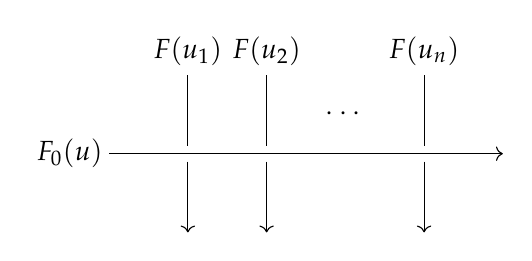
\begin{tikzpicture}[scale=1, transform shape]
    \draw[->] (0,0) -- (5,0);
    \draw[->] (1,-0.1) -- (1,-1);
    \draw[->] (2,-0.1) -- (2,-1);
    \draw[->] (4,-0.1) -- (4,-1);
    \draw[-] (1,0.1) -- (1,1);
    \draw[-] (2,0.1) -- (2,1);
    \draw[-] (4,0.1) -- (4,1);
    \node at (-0.5,0) {$F_0(u)$};
    \node at (1,1.3) {$F(u_1)$};
    \node at (2,1.3) {$F(u_2)$};
    \node at (4,1.3) {$F(u_n)$};
    \node at (3,0.5) {$\cdots$};
\end{tikzpicture}
\end{center}
\caption{Pictorial description of $R_W$}%
\label{fig:}
\end{figure}

Now we have $R_u \in \End(F \otimes W)(u)$, but we wanted elements of $\End(W)$. First, we need to take expansions in $u^{-1}$, and then we view $R_W$ as a matrix with values in $\End(W)$. Finally, we take $Y_Q$ to be generated by all limits (as $u \to \infty$) of all coefficients of all matrix elements of $R_W$ for all possible $F_0$ after dividing by $\hslash$.

Note that $Y_Q$ acts on $F(u_1) \otimes \cdots \otimes F(u_n)$. On the other hand, we had
\[ H_T^*(X(n)^A) \cong F(u_1) \otimes \cdots \otimes F(u_n), \]
because $X(n)^A = X(1)^n$, and therefore $Y_Q$ acts on $H_T^* (X(n))$ for all $n$ because $\on{Stab}_C$ is an isomorphism after localization. This choice should be independent of the choice of $C$ by the Yang-Baxter equation.

Now let $\mf{g}_Q$ be the span of the $u^{-1}$ terms in $Y_Q$ and $\ol{\mf{h}}_Q$ be the span of $\ul{v_i}, \ul{w_i}$, where for $\alpha \in H_T^*(\mc{M}^Q(v, w))$, $\ul{v_i} \cdot \alpha = v_i \cdot \alpha$.

\begin{prop}\leavevmode
    \begin{enumerate}
        \item $\mf{g}_Q$ is a Lie algebra;
        \item $\ol{\mf{h}}_Q \subset \mf{g}_Q$ is a subalgebra;
        \item $\ol{\mf{h}}_Q$ is a maximal commutative subalgebra in $\mf{g}_Q$.
    \end{enumerate}
\end{prop}

\begin{exm}
    Consider $X(2) = \mr{pt} \sqcup T^* \P^1 \sqcup \mr{pt}$. We have
    \begin{align*}
        R(u) &= \frac{1-\frac{\hslash}{u}S}{1-\frac{\hslash}{u}} \\
        &= 1 + \frac{\hslash}{u}(1-S) + O(u^{-2}).
    \end{align*}
    Define $r = 1-S$ to be the classical $r$-matrix. This implies 
    \[ R_W = R_{02}(u-u_2) R_{01}(u-u_1) = 1 + \frac{\hslash}{u}(r_{01} + r_{02}) + O(u^{-2}). \]
    After computation, we will see that $\mf{g}_Q$ is spanned by
    \[ h_1 = \mqty(\dmat{0,1,1,2}), h_2 = \mqty(\dmat{2,1,1,0}), e = \mqty( \\ 1 \\ 1 \\ & 1 & 1 & ), f = \mqty(& 1 & 1 \\ & & & 1 \\ & & & 1 \\ &). \]
    We then see that $h_1 = \ul{u}, h_2 = \ul{w} - \ul{u}$, and that $e, f$ are raising and lowering operators, respectively.
\end{exm}

\begin{prop}
    The associated graded algebra of $Y_Q$ is $\on{gr} Y_Q \simeq \mc{U}(\mf{g}_Q[u])$, where the grading is with respect to degree in $u$ shifted by $1$.
\end{prop}

Then consider $\mf{g}_Q = \ol{\mf{h}}_Q \oplus \bigoplus_{\alpha > 0} (\mf{g}_{\alpha} \oplus \mf{g}_{-\alpha})$.

\begin{thm}
    Let $\lambda \in \C^I$ and $c_1(\lambda) = \sum_{i \in I} \lambda_i c_1(\mc{V}_i)$. Then
    \[ c_1(\lambda) * - = (c_1(\lambda) \cup -) + \hslash \sum_{\alpha > 0} (\lambda, \alpha) \frac{q^{\alpha}}{1-q^{\alpha}} e_{\alpha} \cdot e_{-\alpha} + \cdots, \]
    where the quantum product is modified by $q^{\beta} = (-1)^{(K_X, \beta)} q^{\beta}$.
\end{thm}

Now let $X = \mc{M}^Q(v, w)$. This has an action of $T$, so consider $\gamma \in H_T^2(X)$ and $\gamma_1, \gamma_2 \in H_T^*(X)$. Then we have
\[ (\gamma * \gamma_1, \gamma_2) = (\gamma \cup \gamma_1, \gamma_2) + \sum_{\beta} q^{\beta} \ev{\gamma, \gamma_1, \gamma_2}_{\beta}. \]
But then 
\begin{align*}
    \ev{\gamma, \gamma_1, \gamma_2} &= \qty(\int_{\beta} \gamma) \ev{\gamma_1, \gamma_2}_{\beta} \\
    &= \qty(\int_{\beta} \gamma) \hslash \int_{[\ol{\mc{M}}_{0,2}(X, \beta)]_{\mr{red}}^{\mr{vir}}} \on{ev}^* \gamma_1 \cup \on{ev}^* \gamma_2.
\end{align*}

\chapter{Kevin (Mar 24): Donaldson-Thomas type invariants via microlocal geometry, part 1}%

For any finite type Deligne-Mumford stack $X/\C$, Behrend constructs a natural constructible function $\nu_X$. More precisely, we can use $\nu_X$ to compute enumerative invariants.

\begin{thm}
    Let $X$ be a projective Deligne-Mumford stack (maybe proper with projective coarse moduli space?) with a symmetric obstruction theory. If $X$ is either smooth, a global finite group quotient, or a gerbe over a scheme, then
    \[ \#^{\mr{vir}}(X) = \chi(X, \nu_X) = \sum_{n \in \Z} n \chi(\nu_X^{-1}(n)). \]
\end{thm}

\begin{exm}
    Let $X$ be a DT-type moduli space for a Calabi-Yau threefold. Then $X$ has a symmetric obstruction theory, and so we can compute Donaldson-Thomas and Pandharipande-Thomas invariants for Calabi-Yau threefolds using the Behrend function.
\end{exm}

We will attempt to explain the following diagram where $X \hookrightarrow M$ is an embedding of $X$ into a smooth stack $M$:
\begin{equation}\label{eqn:behrend}
\begin{tikzcd}
    Z_*(X) \ar{r}{\mr{Eu}} \ar[swap]{dr}{c_0^M} & \mr{Con}(X) \ar{d}{c_0^{\mr{SM}}} \ar{r}{\mr{Ch}} & \mc{L}_X(\Omega_M) \ar{dl}{0^!} \\
    & A_0(X).
\end{tikzcd}
\end{equation}
The left triangle was studied by MacPherson, and is relatively well-known. The right triangle is microlocal because of the presence of the cotagent bundle.

\section{Obstruction theories}

\subsection{Perfect obstruction theories}

Recall that a perfect obstruction theory for a Deligne-Mumford stack $X$ is $\phi \colon E \to \tau_{\geq -1} L_X$ that is a surjection on $h^{-1}$ and an isomorphism on $h^0$. We also require that $E$ is a perfect complex with amplitude contained in $[-1, 0]$. Note that $\tau_{\geq -1} L_X$ is locally of the form
\[ [I/I^2 \to \Omega_M |_X], \]
where $M$ is a smooth stack containing $X$.

From the perfect obstruction theory, we can construct the intrinsic normal cone, which is the cone stack $\mf{C}_X$ such that if $U \to X$ is \'etale and $U \to M$ is an embedding into a smooth scheme, then $\mf{C}_X |_U = [C_{U/M} / T_M|_U]$. Then a perfect obstruction theory gives us a closed immersion $\mf{C}_X \hookrightarrow \mf{E}$, and the virtual fundamental class is
\[ [X]^{\mr{vir}} = 0^!_{\mf{E}}(\mf{C}_X) \in A_{\on{rk} E}(X). \]
This is really bad because of the vector bundle stacks, so Behrend gives a different construction that will give us honest vector bundles.

\begin{defn}
    A \textit{local resolution} of $E$ over $U \to X$ is a presentation of $E$ as $[E_1 \to E_0]$ over $U$. The \textit{obstruction cone} is the cone $C$ that is the pullback
    \begin{equation*}
    \begin{tikzcd}
        C \ar[hookrightarrow]{r} \ar{d} & E_1^{\vee} \ar{d} \\
        \mf{C}_{X} |_U \ar[hookrightarrow]{r} & \mf{E} |_U.
    \end{tikzcd}
    \end{equation*}
\end{defn}
We have a surjection $E_1^{\vee} \to \mr{Ob} = H^1(E^{\vee})$.

\begin{prop}
    Let $\Omega$ be a vector bundle on $X$ with a surjection $\Omega \twoheadrightarrow \mr{Ob}$. Then there exists a unique closed subcone $C \subset \Omega$ such that for all local resolutions $[E_0 \to E_0]$ on $U \to X$ with obstruction cone $C'$ and lifts
    \begin{equation*}
    \begin{tikzcd}
        & E_1^{\vee} \ar[twoheadrightarrow]{d} \\
        \Omega |_U \ar{ur}{\phi} \ar[twoheadrightarrow]{r} & \mr{Ob} |_U,
    \end{tikzcd}
    \end{equation*}
    $C|_U = \phi^{-1}(C')$. This $C$ is called the \textit{obstructon cone} of $\Omega \twoheadrightarrow \mr{Ob}$.
\end{prop}

Some nice facts in the case that $X$ is projective are
\begin{itemize}
    \item Perfect obstruction theories admit global resolutions;
    \item There exists an embedding $X \hookrightarrow M$ into a smooth stack.
\end{itemize}

\begin{prop}
    Let $X$ be projective with perfect obstruction theory $E$. Let $\Omega$ be a vector bundle with surjection $\Omega \twoheadrightarrow \mr{Ob}$ and let $C \subset \Omega$ be the obstruction cone. Then $C$ has pure dimension $\on{rk} E + \on{rk} \Omega$ and 
    \[ [X^{\mr{vir}}] = 0^!_{\Omega}(C). \]
\end{prop}

\section{Symmetric obstruction theories}

\begin{defn}
    A \textit{symmetric obstruction theory} is a perfect obstruction theory $E$ endowed with a nondegenerate symmetric bilinear form of degree $1$, which means an isomorphism
    \[ \Theta \colon E \to E^{\vee}[1] \]
    such that $\Theta = \Theta^{\vee}[1]$.
\end{defn}

Note that if $X$ has a symmetric obstruction theory, which means that $[X]^{\mr{{vir}}} \in A_0(X)$. Thus we can define the virtual count $\#^{\mr{vir}}(X) = \deg [X]^{\mr{vir}}$ if $X$ is proper.

\begin{exm}
    Let $Y$ be a projective Calabi-Yau threefold and $X$ be a Hilbert scheme of subschemes of $Y$ of dimension $\leq 1$. Also let $\mc{E}$ be the universal ideal sheaf on $Y \times X$. Then let $\mc{F}$ fit into a distinguished triangle
    \[ \mc{F} \to R\ul{\Hom}(\mc{E}, \mc{E}) \xrightarrow{\tr} \mc{O}_{Y \times X}. \]
    Now $E \coloneqq R \pi_{X*} \mc{F}[2]$ is a symmetric obstruction theory. First, it is clear that $\mc{F}$ is self-dual, and second, by relative Serre duality, we have
    \[ R \pi_* \mc{F}^{\vee}[3] = (R \pi_* \mc{F})^{\vee}. \]
    Shifting and composing, we obtain $E \simeq E^{\vee}[1]$.
\end{exm}

\begin{exm}
    Let $M$ be a smooth variety and let $\omega$ be an almost closed $1$-form (which means that $\dd{\omega}|_{Z(\omega)} = 0)$. Then $X$ has a symmetric obstruction theory
    \[ E = [T_M |_X \to \Omega_M |_X] \qquad v \mapsto \dd(\omega(v)). \]
    This is clearly self-dual, and the map to the cotangent complex is given by $\omega \colon T_M |_X \to I/I^2$. Then we obtain a closed embedding $C_{X/M} \hookrightarrow \Omega_M |_X$, and the image of this is the obstruction cone of $\Omega_M |_X \twoheadrightarrow \mr{Ob}$.
\end{exm}

\begin{prop}
    Let $E$ be a symmetric obstruction theory on $X$. Then \'etale locally, there exists $U \hookrightarrow M$ and an almost closed $1$-form $\omega$ such that $U = Z(\omega)$ and $E|_U$ is the symmetric obstruction theory associated to $\omega$.
\end{prop}

\section{The Behrend function}

We want to think of $\nu_X$ as an invariant of singularities of $X$. This means that:
\begin{itemize}
    \item If $x \in X$ is a smooth point, then $\nu_X(x) = (-1)^{\dim X}$;
    \item If $f \colon X \to Y$ is smooth, then $f^* \nu_Y (-1)^{\dim X - \dim Y} \nu_X$;
    \item For any $x \in X, y \in Y$, we have $\nu_{X \times Y}(x,y) = \nu_X(x) \nu_Y(y)$;
    \item If $X = Z(\dd{f}) \subset M$, then 
        \[ \nu_X(x) = (-1)^{\dim M - 1} \chi ((\Phi_f)_x) = (-1)^{\dim M} (1-\chi(F_x)). \]
        Here, $\Phi_f$ is the vanishing cycles and $F_x$ is the Milnor fiber.
\end{itemize}

Now we want to define $\nu_X$. The first tool is MacPherson's local Euler obstruction
\[ \mr{Eu} \colon Z_*(X) \to \mr{Con}(X), \]
which is in the diagram~\ref{eqn:behrend} and is given by
\[ V \mapsto \qty(x \in V \mapsto \int_{\mu^{-1}(x)} c(\wt{T}) \cap s(\mu^{-1}(x), \wt{V})). \]
Here, if we choose $x \in V$, embed $V \hookrightarrow M$ into a smooth $M$, and consider the Grassmann bundle $G \to V$ of rank $p = \dim V$ quotients of $\Omega_M |_V$. Above the smooth locus $V^s$, there exists a section $V^s \to G$ sending $p$ to $\Omega_V |_p$. Finally, we let $\wt{V}$ be the closure of this section in $G$ and $\mu \colon \wt{V} \to V$ be the natural projection, called the Nash blowup. Also, $\wt{T}$ is the universal quotient bundle on $G$.

Now we can define the Chern-Mather class by
\[ c^M(V) = \mu_* (c(\wt{T}) \cap [\wt{V}]) \in A_*(V). \]

We now need to construct a cycle $\mf{c}_X$. Embed $X \hookrightarrow M$ into a smooth stack and consider the normal cone $C = C_{X/M}$. Also let $\pi \colon C \to X$ be the projection, and define the cycle
\[ \mf{c}_X = \sum_{C'} (-1)^{\dim \pi(C')} \mr{mult}(C') \pi(C'), \]
where $C'$ ranges over the irreducible components of $C$. When $X$ is smooth, then $\mf{c}_X = (-1)^{\dim X} [X]$.

We may finally define the Behrend function by $\nu_X \coloneqq \mr{Eu}(\mf{c}_X)$. There is also the \textit{Aluffi class}
\[ \alpha_X \coloneqq c^M(\mf{c}_X). \]
When $X$ is smooth, then $\alpha_X = c(\Omega_X) \cap [X]$.

\begin{prop}
    In the cases of the main theorem, we have
    \[ \chi(X, \nu_X) = \deg (\alpha_X)_0. \]
\end{prop}

\chapter{Kevin (Mar 31): Donaldson-Thomas type invariants via microlocal geometry, part 2}%

Recall the diagram (\ref{eqn:behrend}) from last time. Our first goal is to show that $(\alpha_X)_0 = [X]^{\mr{vir}}$.

\section{Microlocal geometry}

Let $M$ be a smooth variety of dimension $n$.

\begin{defn}
    An irreducible closed subset $C \subset \Omega_M$ is \textit{conic} if it is invariant under the $\C^*$ action. $C$ is \textit{Lagrangian} if the symplectic form vanishes generically on $C$.
\end{defn}

\begin{defn}
    A closed subscheme of $\Omega_M$ is \textit{conic Lagrangian} if all of its irreducible components of conic Lagrangian.
\end{defn}

Because these conditions are actually \'etale local, we can extend the definitions to the case where $M$ is a smooth Deligne-Mumford stack.

\begin{exm}
    Let $X \subset M$ be irreducible. Then the closure of the conormal bundle to $X^{\mr{sm}}$ is a conic Lagrangian cycle.
\end{exm}

\begin{defn}
    We will define $\mc{L}(\Omega_M) \subset Z_n(\Omega_M)$ to be the group of conic Lagrangian cycles and $\mc{L}_X(\Omega_M)$ to be the group of conic Lagrangian cycles supported over $M$.
\end{defn}

\begin{prop}
    There is an isomorphism $\mc{L}(\Omega_M) \cong Z_*(M)$ given by the maps
    \[ \pi \colon W \mapsto (-1)^{\dim \pi(W)} \pi(W) \]
    and 
    \[ L \colon V \mapsto (-1)^{\dim V} \ol{N^{\vee}_{V^{\mr{sm}}/M}}. \]
\end{prop}

The point of this microlocal geometry is the following result:

\begin{prop}
    The diagram
    \begin{equation*}
    \begin{tikzcd}
        Z_*(X) \ar{r}{L} \ar[swap]{dr}{c_0^M} & \mc{L}_X(\Omega_M) \ar{d}{0^!_{\Omega_M}} \\
        & A_0(X)
    \end{tikzcd}
    \end{equation*}
    commutes.
\end{prop}

\begin{lem}[Fundamental lemma for almost closed $1$-forms]
    The obstruction cone $C$ (where $[X]^{\mr{vir}} = 0^!_{\Omega_M}(C)$) is conic Lagrangian.
\end{lem}

To prove the lemma, we can simply check locally. Now, if we note that
\[ L(\mf{c}_X) = C = C_{X/M} \]
by definition of $\mf{c}_X$, then we obtain
\[ \chi(X, \nu_X) = \int_X c_0^M(\mf{c}_X) = \int_X 0^!_{\Omega_M}(C) = \int_X [X]^{\mr{vir}}, \]
as desired.

\section{Hilbert schemes of points on threefolds}

Let $X = Z(\omega) \subset M$ and $x \in X$. We can choose coordinates $x_1, \ldots, x_n$ on $M$ and extend to coordinates $x_1, \ldots, x_n, p_1, \ldots, p_n$ on $\Omega_M$. Then write
\[ \omega = \sum_i f_i \dd{x_i}. \]
Now let $\eta \in \C - \qty{0}$ and define $\Gamma_{\eta}$ to be the image of $\frac{1}{n} \omega \colon M \to \Omega_M$. We also define $\Delta$ to be the image of the section 
\[ \sum_{i=1}^n \ol{x}_i \dd{x_i} \colon M \to \Omega_M. \]

\begin{prop}
    For $\ep > 0$ small and $\eta$ small relative to $\ep$, we can express the Behrend function as a linking number via the formula
    \[ \nu_X(x) = L_{S_{\ep}} (\Delta \cap S_{\ep}, \Gamma_{\eta} \cap S_{\ep}), \]
    where $S_{\ep}$ is a radius $\ep$ copy of $S^{4n-1}$ around $x \in \Omega_M$.
\end{prop}

We will not consider torus actions. Let $X$ be a $\C^*$-scheme with an isolated fixed point $x$ and an equivariant symmetric obstruction theory.

\begin{prop}
    There exists an invariant affine neighborhood $U \ni x$ where $U = Z(\omega) \subset M$ equivariantly such that $\omega$ is an invariant almost closed $1$-form and $\dim M = \dim T_X |_x$.
\end{prop}

\begin{prop}
    Let $S^1$ act on $S$ with finite stabilizers. Let $A, A', B$ be $S^1$-invariant submanifolds. Suppose we have an $S^1$-equivariant homotopy $T \times Z \to S$ from $A$ to $A'$ where $T$ is an open interval containing $0$ and $1$. Then
    \[ L_S(A, B) = L_S(A', B). \]
\end{prop}

The proof of this requires us to talk about orbifolds, so we will not discuss it.

\begin{prop}
    Let $M$ be a smooth $n$-dimensional $\C^*$ scheme with an isolated fixed point $x$. Let $X = Z(\omega)$, where $\omega$ is an invariant almost closed $1$-form and $x \in X$. Then
    \[ \nu_X(x) = (-1)^n. \]
\end{prop}

\begin{proof}
    Choose equivariant coordinates $x_1, \ldots, x_n, p_1, \ldots, p_n$ on $\Omega_M$ around $x$. Then let
    \[ \Delta_t = \qty{t p_i = \ol{x}_i} \]
    be the image of $(p_1, \ldots, p_n) \mapsto (t \ol{p}_1, \ldots, t \ol{p}_n, p_1, \ldots, p_n)$, which is oriented $(-1)^n$ times the orientation $p_1, \ldots, p_n$. Now let $\Delta_t' = \Delta_t \cap S_{\ep}$. There is an $S^1$-equivariant homotopy from $\Delta_0'$ to $\Delta_1'$ given by the formula
    \[ (t, p_1, \ldots, p_n) \mapsto \frac{\ep}{\sqrt{1+t^2}} (t \ol{p}_1, \ldots, t \ol{p}_n, p_1, \ldots, p_n). \]
    Because $x$ is an isolated fixed points, the action of $S^1$ on $S_{\ep}$ has finite stabilizers, so by the previous proposition,
    \[ L_{S_{\ep}}(\Delta_0', \Gamma_{\eta}') = L_{S_{\ep}}(\Delta_1', \Gamma_{\eta}'). \]
    But the left hand side is $(-1)^n$ and the right side is $\nu_X(x)$, as desired.
\end{proof}

Finally, we give the following result:
\begin{thm}
    For $\C^3$, we have the formula
    \[ \sum_{n=0}^{\infty} \wt{\chi}(\on{Hilb}^n \C^3) t^n = M(-t). \]
\end{thm}

\begin{thm}
    Recall that the fixed points of the torus action on the Hilbert scheme are actually the monomial ideals $I$. But then
    \[ \nu_{\on{Hilb}^n \C^3}(I) = (-1)^{\dim T_{\on{Hilb}} |_I} = (-1)^n \]
    by MNOP, and therefore
    \[ \wt{\chi}(\on{Hilb}^n \C^3) = \sum_I \nu_{\mr{Hilb}}(I) = (-1)^n M_n, \]
    where $M_n$ is the $n$-th coefficient of the McMahon function.
\end{thm}

\chapter{Konstantin (Apr 07): Inductive construction of stable envelopes, part 1}%

\section{Elliptic cohomology}

There is a general way to construct generalized cohomology theories from formal groups using complex cobordism, but this is totally not useful in computations. There is another more explicit construction using derived moduli stacks of elliptic curves, but we don't understand infinity-categories, so it is useless to us. Instead, in 1995, Ginzburg, Kapranov, and Vasserot constructed equivariant elliptic cohomology with complex coefficients. This generalizes a construction of Grojnovski, which reduces to ordinary cohomology in the non-equivariant case. Even here, the notation used by Okounkov (which we will use) is very different from that of Ginzburg, Kapranov, and Vasserot.

We will consider the elliptic curve 
\[ E = \C^{\times} / q^{\Z} \] 
living over $\Spec \C[q]$. This is identified with $\C / \Z + \tau \Z$ by the exponential map $\C \to \C^{\times}$ and $q = e^{2\pi i \tau}$. We will also consider
\[ \mc{E}_z \times \Spec \C[q] \to \Spec \C[q], \]
where $\mc{E}_z$ gives the K\"ahler variables. For an elliptic curve $E$, we have an exact sequence
\[ \Pic^0 E = E^{\vee} \to \Pic E \to NS(E) \cong \Z. \]
Note that any bundle in $\Pic^0(E)$ has a meromorphic section $\frac{\theta(xz)}{\theta(x)}$, where $x \in E, z \in E^{\vee}$, and 
\[ \theta(x) = \prod_{i=1}^{\infty} (1-q^i x) (1-q^{i+1}x^{-1}). \]
This satisfies the equation $\theta(qx) = -x^{-1} \theta(x)$, so we have an entire function on $\C^{\times}$. Also, we note that $\theta(q^n) = 0$, so $\theta(x)$ is a section of the line bundle corresponding to $\qty{0} \subset E$.

Let $G$ be an algebraic group, which for us will be a torus. Then we will define
\[ \ms{Ell}_G(\mr{pt}) \coloneqq G / q^{\on{cochar} G} = E \otimes \on{cochar} G. \]
For example, if $G = (\C^{\times})^n$, then $\ms{Ell}_G(\mr{pt}) = E^n = (\C^{\times})^n / q^{\Z^n}$. In general, we will have a morphism of schemes
\[ \pi \colon \ms{Ell}_G(X) \to \ms{Ell}_G(\mr{pt}). \]
This gives us a sheaf $\pi_* \mc{O}_{\ms{Ell}_G(X)} = \ms{Ell}_G^0(X)$. Note that elliptic cohomology is periodic, and in fact we have
\[ \ms{Ell}_G^{2i}(X) = \ms{Ell}_G^0(X) \otimes \omega^{-i}, \]
where $\omega = \pi^{E,*} T_1 E$ is a line bundle.

\begin{rmk}
    If $G = GL(r)$, then $\ms{Ell}_G(\mr{pt}) = S^r E$. If $G = \mu_r$, then $\ms{Ell}_G(\mr{pt}) = E[r]$ is the group of $r$-torsion points on $E$.
\end{rmk}

\begin{rmk}
    Note that $H_G^{\bullet}(X)$ is a ring over $H_G^{\bullet}(\mr{pt})$. Therefore, we can take $\Spec H_G^{\bullet}(X) = \ms{Lie}(G)$ as a scheme. We can do a similar construction for $\Spec K_G(X) \to \Spec K_G(\mr{pt}) = G$. Then there is a map $\exp \colon \ms{Lie}(G) \to G$, and then of course $\pi \colon G \to G / q^{\on{cochar} G} = \ms{Ell}_G(\mr{pt})$.
\end{rmk}

Now we can construct a sheaf
\[ \pi_*^X \mc{O}_{\ms{Ell}_G(X)} |_U \coloneqq H_G^{\bullet}(X) |_{(\pi \circ \exp)^{-1}(U)}. \]

\begin{exm}
    We will now compute the elliptic cohomology of $X = \P^1$, equivariant with respect to $A = (\C^{\times})^2$. First, note that
    \[ H_A^{\bullet}(\P^1) = \C[u, \alpha_1, \alpha_2] / \ev{(u-\alpha_1)(u-\alpha_2)}. \]
    Note that this is a union of two hyperplanes and projects to $u = 0$. Next, in $K$-theory, we have
    \[ K_A(\P^1) = \C[x^{\pm}, a_1^{\pm}, a_2^{\pm}] / \ev{(1-x^{-1}a_1)(1-x^{-1}a_2)}. \]
    By our choices, we still have a union of hyperplanes, and the projection is onto $x = 1$. We now need to take a quotient with respect to multiplication by $q$, and this tells us that
    \[ \ms{Ell}_A(\P^1) \cong E \cup_{\mr{diag}} E, \]
    where the diagonal is the locus $a_1 = a_2$. In particular, we have
    \[ \mc{O}_{\ms{Ell}_A(\P^1)} = \mc{O}_{\ms{Ell}_{A \times G}(\mr{pt})} / \ev{\theta(x^{-1} a_1) \theta(x^{-1} a_2)}. \]
\end{exm}

Unfortunately, there is no easy geometric interpretations of elliptic cohomology classes comparable to cohomology classes being cycles and $K$-theory classes being sheaves. However, we can consider them as sections of bundles on $\ms{Ell}_G(X)$. Let $V$ be a vector bundle on $X$. Then the \textit{Thom space} of $V$ is defined to be $\mr{Th}(V) = \P(V \oplus \C) / \P(V)$. Its elliptic cohomology is defined to be
\[ \ms{Ell}_G^{\bullet}(\mr{Th}(V)) = \ms{Ell}_G^{\bullet}(\P(V \oplus \C), \P(V)), \]
which is a module over $\mc{O}_{\ms{Ell}_G(X)}$ and thus a pushforward of a sheaf on $\ms{Ell}_G(X)$. We will call this sheaf $\Theta(V)$.

Now denote $\mc{E}_G \coloneqq \ms{Ell}_G(\mr{pt})$ and note that $\ms{Ell}_G(X)$ is a finite cover of $\mc{E}_G$. In cohomology, we have something like
\[ H^{\bullet}(\P(V \oplus \C)) \cong \C[u, v_1, \ldots, v_r, \ldots] / \ev{u \cdot \prod_{i=1}^r (u - v_i)}. \]
This has a map to $H^{\bullet}(\P(V)) = \C[u, v_1, \ldots, v_r, \ldots] / \ev{ \cdot \prod_{i=1}^r (u - v_i)}$, and this tells us that
\[ H^{\bullet}_G(\P(V \oplus \C), \P(V)) = \mc{I} \subset H_G^{\bullet}(\P(V \oplus \C)), \qquad \mc{I} = \ev{\prod (u-v_i)}. \]
Recall from cohomology the Thom isomorphism $H_G^{\bullet}(X) \to H_G(\mr{Th}(V))$ given by $\alpha \to \alpha \prod v_i$. In elliptic cohomology, if we replace $v_i$ by $\theta(v_i)$, we take
\[ \alpha \in \Gamma(\pi^X_* \mc{O}_{\ms{Ell}_G(X)}) \to \alpha \prod \theta(v_i) \in \Gamma (\pi_*^X \Theta(V)). \]

The bundle $\Theta_X(V)$ satisfies the following properties:
\begin{itemize}
    \item $\Theta_X(V \oplus W) = \Theta_X(V) \otimes \Theta_X(W)$;
    \item $\Theta(V^{\vee}) \cong \Theta(V)$.
\end{itemize}
This defines a map $\Theta_X \colon K_G(X) \to \Pic(\ms{Ell}_G(X))$. In fact, this generates all bundles used in Okounkov's constructions.

Now let $f \colon X \to Y$. This defines a map $\ms{Ell}_G(X) \to \ms{Ell}_G(Y)$. We also have a map
\[ f_{\ostar} \in \Hom_{\ms{Ell}_G(Y)}(f_* \Theta_X(-N_f), \mc{O}_{\ms{Ell}_G(Y)}), \]
where $N_f = f^* T Y - T X$. If $f$ is a closed immersion, then $f_{\ostar} \alpha = \alpha \prod_i \theta(v_i)$. On the other hand, if $f$ is a flat projection, we have a fiber integration map
\[ f_{\ostar} \alpha = \frac{\alpha}{\prod \theta(v_i)}. \]

\section{Outline of Okounkov's construction}

Let $(X, \omega)$ be a homomorphic symplectic variety with an action of $T \supset A$, where $A$ preserves the symplectic form. Recall that stable envelopes are related to attracting sets. Recall that if $X^A \subset X$ is the fixed locus, consider characters $w$ entering $N_{X/X^A}$. This defines a hyperplane arrangement in $\mf{a}$, and so we choose a chamber. Each weight becomes a positive, negative, or zero weight of a bundle on $X^A$. This gives us attracting and repelling directions to $X^A$.

For each component $F_i \subset X^A$, we can define $\mr{Attr}(F_i) \subset X \times F_i$ to be the set where $x \in X \to y \in F_i$ as we approach $0 \in \C \supset \C^{\times}$. Next time, we will discuss stable envelopes for elliptic cohomology, which will be sections of bundles that satisfy properties analogous to those of attracting sets.

\chapter{Konstantin (Apr 14): Inductive construction of stable envelopes, part 2}%

\section{More on elliptic cohomology}

Let $G = (\C^{\times})^n$. We again take $E = \C^{\times} / q^{\Z}$. Set
\[ \mc{E}_G \coloneqq \ms{Ell}_G(\mr{pt}) = G/q^{\on{cochar} G}. \]
Recall we have a diagram
\begin{equation*}
\begin{tikzcd}
    \Spec H_G(X) \ar{r}{\mr{ch}} \ar{d} & \Spec K_G(X) \ar{r} \ar{d} & \ms{Ell}_G(X) \ar{d}{\pi^X} \\
    \g \ar{r}{\exp} & G \ar{r} & G/q^{\on{cochar} G}.
\end{tikzcd}
\end{equation*}
We will define the \textit{Elliptic cohomology functor} $X \mapsto \pi_*^X \mc{O}_{\ms{Ell}_G(X)}$. Also recall the Thom sheaf, which was produced from the Thom space
\[ \P(V \oplus \C) / \P(V). \]
This is $\pi_*^X \Theta(-V)$, and $\Theta(V)$ is a line bundle on $\ms{Ell}_G(X)$ with a section $\prod_i \theta(v_i)$.

Finally, recall that if $f \colon X \to Y$ is proper, there is a map
\[ f_{\ostar} \colon f_* \Theta_X(-N_f) \to \mc{O}_{\ms{Ell}_G(Y)}. \]
To construct this, consider the topological picture $X \hookrightarrow V \to Y$ and consider the tubular neighborhood $\mr{Tub}(X)$. Also define $N = T_X V = N_i$, so we have a map $\mr{Th}(V) \to \mr{Th}(N)$. We can also assume that $\mr{Tub}(X) \subset V_{<1}$ is contained inside the disk bundle on $V$. Thus we can assume that
\[ V \setminus \mr{Tub}(X) \supset V \setminus V_{<1}. \]
This defines a map between the elliptic cohomology of $N$ and the elliptic cohomology of $V$, so we obtain
\[ \wt{f}_{\ostar} \colon \pi_*^X \Theta(-N) \to \pi_*^Y \Theta(-V) \]
and then this becomes
\[ \wt{f}_{\ostar} \colon \pi_*^X \Theta(-N + f^* V) \to \pi_*^Y \mc{O}_{\ms{Ell}_G(Y)}, \]
and noting that $\pi_*^X = \pi_*^Y f_*$, we obtain the desired $f_{\ostar}$.

We now discuss correspondences. Consider the diagram
\begin{equation*}
\begin{tikzcd}
    & X \times Y \ar{dl}{p^X} \ar{dr}{p^Y} \\
    X \ar{dr}{\pi^X} & & Y \ar{dl}{\pi^Y} \\
    & \mr{pt}.
\end{tikzcd}
\end{equation*}
Then we want morphisms $\pi_*^X \mc{O}_{\ms{Ell}_G(X)} \to \pi_*^Y \mc{O}_{\ms{Ell}_G(Y)}$. For some class $\alpha$, we will consider the map
\[ p^Y_{\ostar} \alpha p^{X*}(-). \]
To make this work, we require
\[ \alpha \in \Gamma (\Theta(N_{p^Y})) = \Gamma (\Theta(p^{X*} TX)). \]
We can also consider more general line bundles $\mc{S}_X, \mc{S}_Y$ on $\ms{Ell}_G(X), \ms{Ell}_G(Y)$. In this case, we want
\[ \alpha \in \Gamma(\mc{S}_X^{\nabla} \boxtimes \mc{S}_Y), \]
where $\mc{S}^{\nabla} \coloneqq \mc{S}^{-1} \otimes \Theta(TX)$.

\section{Okounkov's construction}

Let $X$ be a holomorphic symplectic variety with symplectic form $\omega$. Let $T$ act on $X$ with $A \subset T$ be the subtorus preserving the symplectic form. Finally, write
\[ X^A = \bigsqcup_{i=1}^N F_i \]
as a disjoint union of connected components. From the bundle $T_{X^A} X = N_{X^A/X}$, we produce characters $w_j$ of $A$ by restricting to each fixed component. Now fix a chamber a chamber $\mc{C} \subset \mf{a} \coloneqq \on{cochar} A \otimes_{\Z} \R$ where every normal weight is either positive or negative. Then if $W$ is a bundle over $X^A$, we of course have
\[ W = W_{>0} \oplus W_{<0} \oplus W_0. \]
For each fixed component, we can define the attracting set $\mr{Attr}(F_i) \subset X$. Now consider the diagram
\begin{equation*}
\begin{tikzcd}
    X \times F_i \ar{d}{p_1} \ar[hookleftarrow]{r}{\jmath} \ar{dr}{p_2} & \mr{Attr}(F_i)  \ar{d}{\pi} \\
    X \ar[hookleftarrow,swap]{r}{\iota} & F_i.
\end{tikzcd}
\end{equation*}
Then note that $N_{\jmath} = \pi^* (N_{<0} + TF)$.

For example, if $X = T^* \P^1$, let $\infty = F_1$ and $0 = F_2$. Then $\mr{Attr}(F_1)$ is the fiber above $\infty$ and $\mr{Attr}(F_2)$ is the base $\P^1 \setminus \infty$. Now define $F_i < F_j$ if $F_i \subset \ol{\mr{Attr}(F_j)}$, and we can upgrade this to a total order, so write $F_1 < F_2 < \cdots < F_N$. Finally, define the total attracting locus
\[ \mr{Attr}^f(F_i) = \bigcup_{j \leq i} \mr{Attr}(F_j). \]
In the example of $X = T^* \P^1$, we see that $\mr{Attr}^f(F_2)$ is the union of the zero section and the fiber above $\infty$. Finally, define
\[ X_i \coloneqq X \setminus \mr{Attr}^f(F_{i-1}). \]
Now define $\mc{S}_A \coloneqq i^* \mc{S} \otimes \Theta(-N_{<0})$.

\begin{prop}
    We have 
    \[ \jmath^* (\mc{S} \boxtimes \mc{S}_A^{\nabla}) \cong \Theta(N_{\jmath}) \]
    for any $\mc{S}$. Thus $\jmath_{\ostar}$ provides a section of $\Theta(N_j)$ on $X_i$.
\end{prop}

\begin{proof}
    We have the identity
    \[ \jmath^* (\mc{S} \boxtimes \mc{S}_A^{\nabla}) = \pi^* (\iota^* \mc{S} \otimes (\iota^* \mc{S} \otimes \Theta(-N_{<0}))). \]
    Then the right hand side becomes
    \[ \pi^* (\Theta(N_{<0}) \otimes \Theta(T F_i)) = \Theta(N_{<0} + T F_i). \qedhere \]
\end{proof}

Now consider the diagram
\begin{equation*}
\begin{tikzcd}
    X_i \times F_i \ar{d}{p_1} \ar[hookleftarrow]{r}{\jmath} & \mr{Attr}(F_i)  \ar{d}{\pi} \\
    X_i \ar[hookleftarrow,swap]{r}{\iota} \ar[hookleftarrow]{ur}{\ol{\jmath}} & F_i.
\end{tikzcd}
\end{equation*}
This defines us a morphism
\[ \ol{\jmath}_{\ostar} \pi^* \colon \Theta(-N_{<0}) \to \mc{O}_{\ms{Ell}_T(X_i)}. \]

\begin{lem}
    The map $\ol{\jmath}_{\ostar} \pi^*$ is injective, so the long exact sequence for the pair $X_i \supset X_{i+1}$ becomes
    \[ 0 \to \Theta(-N_{<0}) \to \mc{O}_{\ms{Ell}_T(X_i)} \to \mc{O}_{\ms{Ell}_T(X_{i+1})} \to 0. \]
\end{lem}

This result gives us an interpolation from $X_{i+1}$ to $X_i$. Tensoring the previous exact sequence with $\mc{S} \boxtimes \mc{S}_A^{\nabla}$ on $X_i \times F_i$, we obtain
\[ 0 \to \iota^* \mc{S} \otimes \Theta(-N_{<0}) \boxtimes \mc{S}_A^{\nabla}|_{F_i} \to \mc{S} \boxtimes \mc{S}_A^{\nabla} |_{X_i} \to \mc{S} \boxtimes \mc{S}_A^{\nabla} |_{X_{i+1}} \to 0. \]
We want to make the support $\Delta$ of $\pi_*^{X_i} (\mc{S}_A |_{F_i} \boxtimes \mc{S}_A^{\nabla} |_{F_j})$ closed on $\mc{E}_T$. If we succeed, we obtain a unique section of $\mc{S} \boxtimes \mc{S}_A^{\nabla} (\infty \Delta)$ (section with poles of arbitrary order at $\Delta$) starting from $\jmath_{\ostar}$ on $X_i \times F_i$. By the inductive construction, we obtain a section on $X \times F_i$.

To make the support closed, we do the following. Let $\mc{L} \to E$ be a line bundle. If $\mc{L}$ has degree $0$, then $H^*(\mc{L}) \neq 0$ if and only if $\mc{L} \cong \mc{O}_E$. Thus we want to make $\deg \mc{S}_A = 0$ over $\mc{E}_A$, which is most simply achieved by polarizations.

\begin{lem}
    If $T^{1/2} \in K_A(X)$ is such that $TX = T^{1/2} + (T^{1/2})^{\vee}$, then we can take $\mc{S} = \Theta(T^{1/2})$.
\end{lem}

This automatically gives us $\deg \mc{S}_A = 0$, and to make $\mc{S}_A$ nontrivial, we can extend the base and take
\[ \mc{S} = \Theta(T^{1/2}) \otimes \mc{U}(\mc{O}_X(1), z), \]
and then $\mc{S}_A$ will be nontrivial for generic $z$.

\chapter{Patrick (Apr 21): DT/PT correspondence using motivic Hall algebras}%

\section{Introduction}

Let $\mc{X}$ be a proper smooth Deligne-Mumford stack with $\omega_{\mc{X}} = \mc{O}_{\mc{X}}$, $H^1(\mc{X}, \mc{O}_{\mc{X}}) = 0$, and projective coarse moduli space $X$. Note here that $X$ is Gorenstein, Calabi-Yau, and has at worst quotient singularities. We will also impose that $\mc{X}$ satisfies the hard Lefschetz condition, which says that age is invariant under the map $I \colon I \mc{X} \to I \mc{X}$ taking $(x, g) \mapsto (x, g^{-1})$.

Now let $N(\mc{X})$ denote the numerical $K$-theory of $\mc{X}$, that is $K(D(\mc{X}))$ modulo the Euler pairing
\[ \chi(E, F) = \sum (-1)^i \dim \Ext^i_{\mc{X}}(E, F). \]
Then denote $N_{\leq 1}(\mc{X})$ denote the classes with support in dimension at most $1$ and $N_0(\mc{X})$ be the classes with $0$-dimensional support. Then choose\footnote{For a manifold, $\on{ch}_3$ defines a canonical splitting, but this cannot always be done for orbifolds.} a splitting
\[ N_{\leq 1}(\mc{X}) = N_1(\mc{X}) \oplus N_0(\mc{X}) \ni (\beta, c). \]
Finally, we call a class $\beta \in N_1(\mc{X})$ \textit{effective} if it is represented by an actual sheaf $F \in \mt{Coh}_{\leq 1}(\mc{X})$.

Now let $Y = \on{Quot}(\mc{O}_{\mc{X}}, [\mc{O}_x])$ for a non-stacky point $x \in \mc{X}$. Then $Y$ is a smooth projective Calabi-Yau threefold and there is a map $f \colon Y \to X$, which is a crepant resolution. Then, if we consider the universal sheaf on $Y \times \mc{X}$ by $\mc{O}_{\mc{Z}}$, the Fourier-Mukai transform
\[ \Phi = p_{\mc{X}*} (\mc{O}_{\mc{Z}} \otimes p_Y^*(-)) \colon D(Y) \to D(\mc{X}) \]
is a derived equivalence, called the \textit{McKay correspondence}. Then there is a map $N_{\leq 1}(Y) \to N_{\leq 1}(\mc{X})$, and thus we obtain a splitting $N_{\leq 1}(Y) = N_{\text{n-exc}}(Y) \oplus N_{\mr{exc}}(Y)$. Finally, write $N_{\mr{mr}}(\mc{X}) = \Phi(N_{\leq 1}(Y))$ and $N_{1,\mr{mr}}(\mc{X}) = \Phi(N_{\text{n-exc}}(Y))$. Also, write $\Psi \coloneqq \Phi^{-1}$.

Then define following DT and PT generating series:
\begin{align*}
    \mr{DT}(\mc{X})_{\beta} &= \sum_{c \in N_0(\mc{X})} \mr{DT}(\mc{X})_{(\beta, c)} q^c; \\
    \mr{DT}(\mc{X})_{0} &= \sum_{c \in N_0(\mc{X})} \mr{DT}(\mc{X})_{(0, c)} q^c; \\
    \mr{PT}(\mc{X})_{\beta} &= \sum_{c \in N_0(\mc{X})} \mr{PT}(\mc{X})_{(\beta, c)} q^c.
\end{align*}

\begin{thm}[DT/PT correspondence]
    Let $\beta \in N_{1, \mr{mr}}(\mc{X})$. Then there is an equality of generating series
    \[ \mr{PT}(\mc{X})_{\beta} = \frac{\mr{DT}(\mc{X})_{\beta}}{\mr{DT}(\mc{X})_0}. \]
\end{thm}

\section{Categorical preliminaries}

\begin{defn}
    Let $\mt{B}$ be an abelian category. Then a \textit{torsion pair} is a pair of full subcategories $(\mt{T}, \mt{F})$ such that $\Hom(T, F) = 0$ for all $T \in \mt{T}, F \in \mt{F}$ and every $E \in \mt{B}$ fits into a (unique) short exact sequence
    \[ 0 \to T_E \to E \to F_E \to 0 \]
    with $T_E \in \mt{T}, F_E \in \mt{F}$.
\end{defn}
This can be naturally generalized to the notion of a \textit{torsion $n$-tuple} $(\mt{B}_1, \ldots, \mt{B}_n)$.

\begin{exm}
    Let $\mt{T} = \mt{Coh}_{\leq d}(\mc{X})$ and $\mt{F} = \mt{Coh}_{\geq d+1}(\mc{X})$ be the category of sheaves with no subsheaves of dimension $\leq d$. Then $(\mt{T}, \mt{F})$ is a torsion pair on $\mt{Coh}(\mc{X})$.
\end{exm}

For a torsion pair $(\mt{T}, \mt{F})$, we can define a new abelian category 
\[ \mt{B}^{\flat} = \qty{E \in D^{[-1,0]}(\mt{B}) \mid H^{-1}(E) \in \mt{F}, H^0(E) \in \mt{T}}. \]
This is called \textit{tilting} at the torsion pair $(\mt{T}, \mt{F})$.

\begin{exm}
    Define the category $\mt{Coh}^{\flat}(\mc{X})$ by tilting at the torsion pair of the previous example for $d = 1$.
\end{exm}

Unfortunately, this category is too large for our purposes, so we will define a new category. First, if $\mc{C}_1, \ldots, \mc{C}_n \subset D(\mc{X})$ are full subcategories, let $\ev{\mc{C}_1, \ldots, \mc{C}_n}_{\mr{ex}} \subset D(\mc{X})$ be the smallest full subcategory of $D(\mc{X})$ containing all of the $\mc{C}_i$ and closed under extensions. Now we may define 
\[ \mt{A} = \ev{\mc{O}_{\mc{X}}[1], \mt{Coh}_{\leq 1}(\mc{X})}_{\mr{ex}} \subset \mt{Coh}^{\flat}(\mc{X}). \]
This is a Noetherian abelian category with the inclusions $\mt{Coh}_{\leq 1}(\mc{X}) \subset \mt{A} \subset D(\mc{X})$ being exact. In addition, $\mt{A}$ contains all ideal sheaves $I_C[1]$, PT stable pairs, and Bryan-Steinberg pairs.

\begin{defn}
    Let $\mt{T}, \mt{F}$ be full subcategories of $\mt{Coh}_{\leq 1}(\mc{X})$. Write $\mt{Pair(T,F)} \subset \mt{A}$ for the full subcategory on objects $E$ such that $\on{rk} E = -1$, $\Hom(T, E) = 0$ for $T \in \mt{T}$, and $\Hom(E, F) = 0$ for $F \in \mt{F}$. 
\end{defn}

\begin{exm}
    For example, if $\mt{T}_{\mr{PT}} = \mt{Coh}_0(\mc{X})$ and $\mt{F}_{\mr{PT}} = \mt{Coh}_{1}(\mt{X})$, then a $(\mt{T}_{\mr{PT}}, \mt{F}_{\mr{PT}})$-pair is a PT stable pair.
\end{exm}

For a pair of full subcategories as above, we may also define
\[ \mt{V(T,F)} \coloneqq \qty{E \in \mt{A} \mid \Hom(\mt{T}, E) = \Hom(E, \mt{F}) = 0}. \]
If $(\mt{T}, \mt{F})$ and $(\wt{\mt{T}}, \wt{\mt{F}})$ are torsion pairs, then $(\mt{T}, \mt{V(T, \wt{F})}, \wt{\mt{F}})$ is a torsion triple on $\mt{A}$.

\section{Moduli stack}

There is a stack $\mf{Mum}_Y$ parameterizing objects $E \in D(Y)$ such that $\Ext^{<0}(E, E) = 0$ which is an Artin stack locally of finite type, which was constructed by Lieblich in 2006.\footnote{As with all students of Johan, this was actually done in maximal generality for a proper morphism of algebraic spaces.} Because Fourier-Mukai transforms behave well in families, by the McKay correspondence, we have a corresponding stack $\mf{Mum}_{\mc{X}}$. In addition, there is a decomposition
\[ \mf{Mum}_{\mc{X}} = \bigsqcup_{\alpha \in N(\mc{X})} \mf{Mum}_{\mc{X}, \alpha} \]
into open and closed substacks by the numerical $K$-theory class. If $\mt{C} \subset D(\mc{X})$ is a full subcategory of objects with vanishing self-$\Ext^{<0}$ and defines an open substack of $\mf{Mum}_{\mc{X}}$, then we will call the corresponding open substack $\mt{\ul{C}} \subset \mf{Mum}_{\mc{X}}$.

\begin{defn}
    A torsion pair $(\mt{T}, \mt{F})$ on $\mt{Coh}_{\leq 1}(\mc{X})$ is \textit{open} if $\mt{T}, \mt{F}$ are open subcategories.
\end{defn}

\begin{lem}
    The following conditions define open substacks of $\mf{Mum}_{\mc{X}}$ for full, open subcategories $\mt{T}, \mt{F}$ of $\mt{Coh}(\mc{X})$:
    \begin{enumerate}
        \item $H^0(E) \in \mt{T}$ and $E \in D^{[-1,0]}(\mc{X})$;
        \item $H^{-1}(E) \in \mt{F}$ and $E \in D^{[-1,0]}(\mc{X})$.
    \end{enumerate}
    In particular, if $(\mt{T}, \mt{F})$ is an open torsion pair, then the objects of the tilt of $\mt{Coh}(\mc{X})$ at $(\mt{T}, \mt{F})$ form an open substack of $\mf{Mum}_{\mc{X}}$
\end{lem}

\begin{prop}
    Let $(\mt{T}, \mt{F})$ be open torsion pairs on $\mt{Coh}_{\leq 1}(\mc{X})$. Suppose that $\mt{Coh}_0(\mc{X}) \subset \mt{T}$. Then the substack $\mt{\ul{Pair}(T, \wt{F})} \subset \mf{Mum}_{\mt{X}}$ is open.
\end{prop}

In particular, $\mt{Coh}^{\flat}(\mc{X})$ is an open subcategory. In addition, the category $\mt{A}_{\on{rk}\geq -1} \subset \mt{Coh}^{\flat}(\mc{X})$ is open. This means that
\[ \mt{\ul{A}}_{\on{rk} \geq -1} \subset \ul{\mt{Coh}}^{\flat}(\mc{X}) \subset \mf{Mum}_{\mc{X}} \]
are inclusions of open substacks, and in particular, the first two stacks are Artin stacks locally of finite type.

\section{Motivic Hall algebras}

Recall the Grothendieck ring of varieties $K(\mt{Var}_{\C})$ (taken with $\Q$-coefficients), which is spanned by isomorphism classes of varieties with the relations $[X] = [Z] + [X \setminus Z]$ for a closed subvariety $Z \subset X$ and $[X] \cdot [Y] = [X \times Y]$. This will not be helpful when we consider stacks, so instead we will consider the following two relations.

\begin{defn}
    Let $Y$ be connected. Then a morphism $f \colon X \to Y$ is a \textit{Zariski fibration} if there is an open cover $Y = \bigcup U_i$ such that $f^{-1}(U_i) = U_i \times F_i$.\footnote{Given our assumptions, all $F_i$ are isomorphic.}
\end{defn}

\begin{defn}
    A morphism $f \colon X \to Y$ is a \textit{geometric bijection} if $f$ induces a bijection on $\C$-points.
\end{defn}

\begin{lem}
    $K(\mt{Var}_{\C})$ is spanned by isomorphism classes of varieties with the following relations:
    \begin{enumerate}
        \item If $f \colon X \to Y$ is a geometric bijection, then $[X] = [Y]$;
        \item $[X_1] + [X_2] = [X_1 \sqcup X_2]$.
    \end{enumerate}
\end{lem}

Now we say that a morphism $f \colon X \to Y$ of stacks is a Zariski fibration if for any scheme $T$, the base change $f_T \colon X \times_{Y} T \to T$ is a Zariski fibration of schemes. Of course, the definition of geometric bijection should be changed to that of inducing an equivalence on groupoids of $\C$-points.

\begin{defn}
    The \textit{Grothendieck ring of stacks} $K(\mt{St}_{\C})$ is the $\Q$-vector space spanned by symbols $[X]$ for finite type Artin stacks with affine stabilizers $X$ with the following relations:
    \begin{enumerate}
        \item $[X \sqcup Y] = [X] + [Y]$;
        \item If $f \colon X \to Y$ is a geometric bijection, then $[X] = [Y]$;
        \item If $X_1, X_2 \to Y$ are Zariski fibrations with the same fibers, then $[X] = [Y]$.
    \end{enumerate}
\end{defn}
For any Artin stack $S$ locally of finite type with affine stabilizers, then there is a relative version $K(\mt{St}_S)$, which is a module over $K(\mt{St}_{\C})$. For our purposes, we will take $\mt{C} = \mt{Coh}^{\flat}(\mc{X})$ and let $S = \mt{\ul{C}}$. 

\begin{prop}
    There exists an Artin stack $\mt{\ul{C}}^{(2)}$ locally of finite type parameterizing short exact sequences in $\mt{C}$. This stack is equipped with maps
    \[ \pi_i \colon \mt{\ul{C}}^{(2)} \to \mt{\ul{C}} \qquad [0 \to E_1 \to E_2 \to E_3 \to 0] \mapsto E_i \]
    for $i = 1,2,3$. Then the morphism $(\pi_1, \pi_3) \colon \mt{\ul{C}}^{(2)} \to \mt{\ul{C}}$ is of finite type.
\end{prop}

Now, for $[X_1 \to \mt{\ul{C}}], [X_2 \to \mt{\ul{C}}] \in K(\mt{St}_{\mt{\ul{C}}})$, define the stack $X_1 * X_2$ as the fiber product
\begin{equation*}
\begin{tikzcd}
    X_1 * X_2 \ar{r} \ar{d} & \mt{\ul{C}}^{(2)} \ar{r}{\pi_2} \ar{d}{(\pi_1, \pi_3)} & \mt{\ul{C}} \\
    X_1 \times X_2 \ar{r} & \mt{\ul{C}} \times \mt{\ul{C}}.
\end{tikzcd}
\end{equation*}
This defines an associative product on $K(\mt{St}_{\mt{\ul{C}}})$, and we define the \textit{motivic Hall algebra} $H(\mt{C}) \coloneqq (K(\mt{St}_{\mt{\ul{C}}}), *)$.

There is an inclusion $K(\mt{Var}_{\C})[\L^{-1}, (1 + \cdots + L^n)^{-1} \mid n \geq 1] \to K(\mt{St}_{\C})$. Then we define the subalgebra of \textit{regular elements} $H_{\mr{reg}}(\mt{C})$ to be the $K(\mt{Var}_{\C})[\L^{-1}, [\P^n]^{-1} \mid n \geq 1]$-submodule generated by schemes $[Z \to \mt{\ul{C}}]$.

\begin{prop}
    $H_{\mr{reg}}(\mt{C})$ is closed under $*$ and the quotiennt $H_{\mr{reg}}(\mt{C}) / (\L - 1) H_{\mr{reg}}(\mt{C})$ is commutative with Poisson bracket given by $\qty{f, g} = \frac{f * g - g * f}{\L - 1}$. This is called the \textit{semi-classical Hall algebra}.
\end{prop}

Let $\Q[N(\mc{X})]$ with product $t^{\alpha_1} \star t^{\alpha_2} = (-1)^{\chi(\alpha_1, \alpha_2)} t^{\alpha_1 + \alpha_2}$ be the \textit{Poisson torus}. The Poisson bracket is defined by $\qty{t^{\alpha}, t^{\beta}} = (-1)^{\chi(\alpha, \beta)} \chi(\alpha, \beta) t^{\alpha + \beta}$. Then there is a Poisson algebra homomorphism
\[ I \colon H_{\mr{sc}}(\mt{C}) \to \Q[N(\mc{X})] \qquad [s \colon Y \to \mt{C}_{\alpha} \hookrightarrow \mt{C}] = e(Y, s^{-1} \nu), \]
where $\nu \colon \mt{C} \to \Z$ is the Behrend function.

We will not be considering the motivic Hall algebra but rather a completed version $H_{\mr{gr}}(\mt{C})$ which is analogous to the completion from Laurent polynomials to Laurent series. There is an algebra $H_{\mr{gr,reg}}(\mt{C})$ of regular elements and a semi-classical algebra $H_{\mr{gr,sc}}(\mt{C})$, which comes with an integration morphism 
\[ I \colon H_{\mr{gr,sc}}(\mt{C}) \to \Q \qty{N(\mc{X})} = \qty{\sum_{\alpha \in N(\mc{X})} n_{\alpha} t^{\alpha}}. \]

\section{Wall-crossing and the DT/PT correspondence}

\begin{defn}
    A torsion pair $(\mt{T}, \mt{F})$ on $\mt{Coh}_{\leq 1}(\mc{X})$ is called \textit{numerical} if whenever $[T \in \mt{T}] = [F \in \mt{F}]$ in $N(\mc{X})$, then $T = F = 0$.
\end{defn}
All of the torsion pairs we will consider are numerical.

\begin{prop}
    Let $(\mt{T}, \mt{F})$ be an open numerical torsion pair and suppose that $\mc{M} \subset \mt{\ul{Pair}(T,F)}$ is an open and finite type substack. Then $(\L - 1) [\mc{M}] \in H_{\mr{reg}}(\mt{C})$.
\end{prop}

\begin{lem}
    Assume that $\mt{Pair(T_-, F_-)}, \mt{Pair(T_+, F_+)}, \mt{W}$ define elements of $H_{\mr{gr}}(\mt{C})$ and let $\alpha \in N(\mt{A})$. The following are equivalent:
    \begin{enumerate}
        \item The stack $\mt{\ul{Pair}(T_+, F_-)}_{\alpha}$ is of finite type.
        \item The stack $(\mt{\ul{Pair}(T_+, F_+)} * \mt{\ul{W}})_{\alpha}$ is of finite type.
        \item The stack $(\mt{\ul{W}} * \mt{\ul{Pair}(T_-, F_-)})_{\alpha}$ is of finite type.
    \end{enumerate}
\end{lem}

\begin{defn}
    A full subcategory $\mt{W} \subset \mt{Coh}_{\leq 1}(\mc{X})$ is \textit{log-able} if
    \begin{enumerate}
        \item $\mt{W}$ is closed under direct sums and summands;
        \item $\mt{W}$ defines an element of $H_{\mr{gr}}(\mt{C})$;
        \item If $\alpha \in N(\mc{X})$, there are only finitely many ways to write $\alpha = \alpha_1 + \cdots + \alpha_n$, where each $\alpha_i$ represents a nonzero element in $\mt{W}$.
    \end{enumerate}
\end{defn}

\begin{thm}[No-poles]
    If $\mt{W}$ is log-able, then
    \[ (\L - 1) \log [\mt{\ul{W}}] \in H_{\mr{gr,reg}}(\mt{C}). \]
\end{thm}

We are finally ready to do wall-crossing, but we need one more definition.

\begin{defn}
    Let $(\mt{T}_{\pm}, \mt{F}_{\pm})$ be open torsion pairs on $\mt{Coh}_{\leq 1}(\mc{X})$ such that $\mt{T}_+ \subset \mt{T}_-$. Let $\mt{W} = \mt{T}_- \cap \mt{F}_+$. These torsion pairs are \textit{wall-crossing material} if $\mt{W}$ is log-able and the categories $\mt{Pair(T_+, F_-)}, \mt{Pair(T_-, F_+)}, \mt{Pair(T_+,F_-)}$ define elements of $H_{\mr{gr}}(\mt{C})$.
\end{defn}

\begin{thm}
    Suppose $(\mt{T_{\pm}}, \mt{F_{\pm}})$ are open torsion pairs with $\mt{T_+} \subset \mt{T_-}$ which are wall-crossing material. Then $w \coloneqq I((\L-1) \log [\mt{\ul{W}}])$ is well-defined and
    \[ I((\L-1)[\mt{\ul{Pair}(T_+,F_+)}]) = \exp(\qty{w,-}) I((\L-1) [\mt{\ul{Pair}(T_-, F_-)}]). \]
\end{thm}

\begin{proof}[Proof of DT/PT correspondence]
    Let $\mt{T}_{\mr{DT}} = 0, \mt{F}_{\mr{DT}} = \mt{Coh}_{\leq 1}(\mc{X}), \mt{W} = \mt{Coh}_0(\mt{X})$. Then the torsion pairs $(\mt{T}_{\mr{DT}}, \mt{F}_{\mr{DT}}), (\mt{T}_{\mr{PT}}, \mt{F}_{\mr{PT}})$ are wall-crossing material, so we can apply the previous theorem. Isolating the terms with class $\beta$ and noting that $(\mt{T}_{\mr{DT}}, \mt{F}_{\mr{DT}})$-pairs are ideal sheaves $I[1]$, we obtain
    \[ \mr{DT}(\mc{X})_{\beta}z^{\beta} t^{-[\mc{O}_{\mc{X}}]} = \exp(\qty{w,-}) \mr{PT}(\mc{X})_{\beta} z^{\beta} t^{-[\mc{O}_{\mc{X}}]}. \]
    Now let $c \in N_0(\mc{X})$. Applying the McKay equivalence, we have $\Psi(c) \in N_{\leq 1}(Y)$. Because $\beta$ is multi-regular, $\Psi(\beta, c') \in N_{\leq 1}(Y)$ for all $c' \in N_0(\mc{X})$. But then the Euler pairing is trivial on $N_{\leq 1}(Y)$, so 
    \[ \chi(c, (\beta, c')) = \chi(\Psi(c), \Psi(b, c')) = 0. \]
    Next, write $w = \sum_{c \in N_0(\mc{X})} w_c q^c$. We then have $\qty{w, z^{\beta}q^{c'}} = 0$, so
    \[ \exp(\qty{w, -}) \mr{PT}(\mc{X})_{\beta} z^{\beta} t^{-[\mc{O}_{\mc{X}}]} = PT(\mc{X})_{\beta} z^{\beta} \exp(\qty{w,-}) t^{-[\mc{O}_{\mc{X}}]}. \]
    Combining this with the first DT-PT identity, we have 
    \[ \frac{\mr{DT}(\mc{X})_{\beta}}{\mr{PT}(\mc{X})_{\beta}} = t^{[\mc{O}_{\mc{X}}]} \exp(\qty{w,-}) t^{-[\mc{O}_{\mc{X}}]}. \]
    Finally, noting that $\mr{PT}(\mc{X})_0 = 1$ because $\mc{O}_{\mc{X}}[1]$ is the only stable pair with $\beta = 0$, we obtain
    \[ \frac{\mr{DT}(\mc{X})_{\beta}}{\mr{PT}(\mc{X})_{\beta}} = \frac{\mr{DT}(\mc{X})_{0}}{\mr{PT}(\mc{X})_{0}} = \mr{DT}(\mc{X})_{0}. \qedhere \]
\end{proof}

\chapter{Patrick (Apr 28): The DT crepant resolution conjecture}%

\section{Brief review}

Recall that $\mc{X}$ is a projective Calabi-Yau 3-orbifold (where we require $H^1(\mc{O}_{\mc{X}} = 0)$), that $X$ is the coarse moduli space (which is a projective, Gorenstein, Calabi-Yau variety with at worst quotient singularities), and $Y$ was a distinguished crepant resolution of $X$. Also recall that we have derived equivalences $\Phi \colon D(Y) \leftrightarrow D(\mc{X}) \colon \Psi$.

Let $\mt{C}$ be the category $\mt{Coh}(\mc{X})$ tilted at the torsion pair $(\mt{Coh}_{\leq 1}(\mc{X}), \mt{Coh}_{\geq 2}(\mc{X}))$. We consider the graded motivic Hall algebra $H_{\mr{gr}}(\mt{C})$, which is a module over $K(\mt{St}_{\C})$. Also, recall the category
\[ \mt{A} = \ev{\mc{O}_{\mc{X}}[1], \mt{Coh}_{\leq 1}(\mc{X})}. \]
Finally, recall the integration map $I \colon H_{\mr{gr,sc}}(\mt{C}) \to \qty{\sum_{\alpha \in N(\mc{X})} n_{\alpha} q^{\alpha}}$, where $H_{\mr{sc}}(\mt{C})$ is a quotient of the algebra 
\[ H_{\mr{reg}}(\mt{C}) = K(\mt{Var}_{\C})[\L^{-1}][[\P^n]^{-1} \mid n \geq 1] \cdot \qty{\text{schemes}} \subset H(\mt{C}). \]
of regular elements.

\section{Stability conditions}

Fix an ample class $\omega \in N^1(Y)$ and an ample line bundle $A$ on $X$.

\begin{defn}
    A \textit{stability condition} on $\mt{Coh}_{\leq 1}(\mc{X})$ consists of a slope function $\mu \colon N_{\leq 1}(\mc{X}) \to S$ to a totally ordered set $(S, <)$ such that if
    \[ 0 \to A \to B \to C \to 0, \]
    then either $\mu(A) > \mu(B) > \mu(C)$ or $\mu(A) < \mu(B) < \mu(C)$ or $\mu(A) = \mu(B) = \mu(C)$ and every $F \in \mt{Coh}_{\leq 1}(\mc{X})$ has a Harder-Narasimhan filtration $0 = F_0 \subset \cdots \subset F_n = F$.
\end{defn}

We will now define a number of stability conditions. First, we fix a ``generating'' vector bundle $V$ (where every coherent sheaf on $\mc{X}$) is locally a quotient of $V^{\oplus n}$ for some $n$. We can assume that $V = V^{\vee}$ (by taking $V \oplus V^{\vee}$). Now we define a modified Hilbert polynomial for a sheaf $F$ by
\[ p_F(k) = \chi(\mc{X}, V^{\vee} \otimes F(k)) = \ell(F) k + \deg(F). \]

\begin{defn}
    Define the \textit{Nironi slope} of $F$ to be
    \[ \nu(F) \coloneqq \frac{\deg F}{\ell(F)} \]
    if $F \notin \mt{Coh}_0(\mc{X})$ and $\nu(F) = \infty$ otherwise. Also write $\nu_+(F), \nu_-(F)$ for the slopes of the Harder-Narasimhan factor of $F$ with largest (resp. smallest) slope.
\end{defn}

\begin{defn}
    Define the stability condition $\zeta$ on $N_1^{\mr{eff}}(\mc{X}) \setminus 0$ by
    \[ \zeta(\beta, c) = \qty(- \frac{\deg_Y(\on{ch_2}(\Psi(A \cdot \beta)) \cdot \omega)}{\deg(A \cdot \beta)}, \nu(\beta, c)) \in (-\infty, \infty]^2 \]
    for $\beta = 0$ and $\zeta(0, c) = (\infty, \infty)$. Here, we use the lexicographical ordering on $(-\infty, \infty]$.
\end{defn}

For a stability condition $\mu$ and $s \in S$, define a torsion pair by 
\begin{align*}
    \mt{T}_{\mu, s} &\coloneqq \qty{T \in \mt{Coh}_{\leq 1}(\mc{X}) \mid T \twoheadrightarrow Q \neq 0 \implies \mu(Q) \geq s}; \\
    \mt{F}_{\mu, s} &\coloneqq \qty{F \in \mt{Coh}_{\leq 1}(\mc{X}) \mid 0 \neq H \hookrightarrow F \implies \mu(H) < s}.
\end{align*}
Also, call the category of $(\mt{T}_{\mu, s}, \mt{F}_{\mu, s})$-pairs $\mt{P}_{\mu, s}$. Finally, define the category of semistable sheaves of slope $s$ by $\mc{M}_{\mu}^{\mr{ss}}(s)$.

In order to control DT-like invariants coming from stability conditions, we need our categories of semistable objects and of pairs to satisfy openness and boundedness properties. 

\begin{prop}\leavevmode
    \begin{enumerate}
        \item For any $\delta \in \R$, the torsion pair $(\mt{T}_{\nu,\delta}, \mt{F}_{\nu, \delta})$ is open.
        \item For any $(\gamma, \eta) \in \R_{>0} \times \R$, the torsion pair $(\mt{T}_{\zeta, (\gamma,\eta)}, \mt{F}_{\zeta, (\gamma,\eta)})$ is open. In addition, the moduli stack $\ul{\mc{M}}_{\zeta}^{\mr{ss}}(a,b) \subset \mt{\ul{Coh}}_{\leq 1}(\mc{X})$ is open for any $(a,b) \in \R^2$.
    \end{enumerate}
\end{prop}

We will now discuss boundedness. For any real number $\gamma > 0$, define the function
\[ L_{\gamma} \colon N_0(\mc{X}) \to \R \qquad c \mapsto \deg(c) + \gamma^{-1} \deg_Y(\on{ch_2}(\Psi(c)) \cdot \omega). \]
This will control the series expansion of the rational function $f_{\beta}(q)$, where $\mr{PT}(\mc{X})_{\beta}$ is the expansion of $f_{\beta}(q)$ in $\Q[N_0(\mc{X})]_{\mr{deg}}$ (this means roughly that degree is bounded below).

\begin{defn}
    Let $S \subset N_0(\mc{X})$ and $L \colon N_0(\mc{X}) \to \R$ be a homomorphism. Then $S$ is \textit{$L$-bounded} if the set
    \[ S \cap \qty{c \in N_0(\mc{X}) \mid L(c) \leq M} \]
    is finite for every $M \in \R$. We also say that $S$ is \textit{weakly $L$-bounded} if the set
    \[ (S/\ker L) \cap \qty{c \in N_0(\mc{X})/L \mid L(c) \leq M} \]
    is finite for every $M \in \R$.
\end{defn}

The main results about semistable sheaves and pairs are the following. Recall that a category $\mt{W}$ is log-able if $(\L-1) \log[\mt{\ul{W}}] \in H_{\mr{gr,reg}}(\mt{C})$.
\begin{prop}
    Let $(a,b) \in \R^2$. The set
    \[ \qty{ c \in N_0(\mc{X}) \mid \ul{\mc{M}}^{\mr{ss}}(a,b) \neq \emptyset} \]
    is $L_{\gamma}$-bounded. Moreover, the category $\mc{M}_{\gamma}^{\mr{ss}}(a, b)$ is log-able.
\end{prop}

\begin{prop}
    For any $(\gamma, \eta) \in \R_{>0} \times \R$, the set
    \[ \qty{c \in N_0(\mc{X}) \mid \mt{P}_{\zeta, (\gamma, \eta)}(\beta, c) \neq \emptyset} \]
    is $L_{\gamma}$-bounded. Moreover, the stack $\mt{\ul{P}}_{\zeta, (\gamma,\eta)}(\beta, c)$ is of finite type.
\end{prop}

\begin{cor}
    The category $\mt{P}_{\zeta, (\gamma, \eta)}$ defines an element of $H_{\mr{gr}}(\mt{C})$.
\end{cor}

Finally, we will locate regions in which the notion of a $(\mt{T}_{\zeta,(\gamma,\eta)}, \mt{F}_{\zeta, (\gamma,\eta)})$-pair is constant.

\begin{lem}
    Let $\beta \in N_1(\mc{X})$. $\mt{T}_{\gamma,(\gamma,\eta)} \cap \mt{Coh}_{\leq 1}(\mc{X})_{\leq \beta}$ and $\mt{F}_{\zeta, (\gamma,\eta)} \cap \mt{Coh}_{\leq 1}(\mc{X})_{\leq \beta}$ are constant on the components of $(\R_{>0} \times \R) \setminus (V_{\beta} \times \R)$, where
    \[ V_{\beta} = \qty{- \frac{\deg_Y(\on{ch}_2(\Psi(A \cdot \beta')) \cdot \omega)}{\deg(A \cdot \beta')} \mid 0 < \beta' \leq \beta} \cap \R_{>0}. \]
    For $\gamma \in V_{\beta}$, the categories are locally constant on $\qty{\gamma} \times \R \setminus W_{\beta}$, where $W_{\beta} = \frac{1}{\ell(\beta)!} \Z$.
\end{lem}

\section{DT-like invariants}

We define DT-like invariants counting objects in the categories that we have defined. Once we do this, we will cross our infinitely many walls.

Recall that $\mc{M}_{\zeta}^{\mr{ss}}(a, b)$ is log-able for any $(a, b) \in \R^2$. Therefore, we have an element
\[ \eta_{\zeta, (a,b)} = (\L-1) \log [\ul{\mc{M}}_{\zeta}^{\mr{ss}}(a,b)] \in H_{\mr{gr, reg}}(\mt{C}). \]
Therefore, we can define DT-type (Joyce-Song) invariants by
\[ \sum_{\zeta(\beta, c) = (a,b)} J_{(\beta,c)}^{\zeta} z^{\beta} q^c \eqqcolon I\qty(\eta_{\zeta,(a,b)}). \]

Now let $(\gamma, \eta) \in \R_{>0} \times \R$ be away from the walls. By a result of Abramovich-Corti-Vistoli, there is an element $(\L-1)[\mt{\ul{P}}_{\zeta,(\gamma,\eta)}(\beta, c)] \in H_{\mr{reg}}(\mt{C})$. Then we can define DT-type invariants by
\[ \mr{DT}_{(\beta,c)}^{\zeta,(\gamma,\eta)}z^{\beta} q^c t^{-[\mc{O}_{\mc{X}}]} \coloneqq I((\L-1)[\mt{\ul{P}}_{\zeta,(\gamma,\eta)}(\beta,c)]). \]
Finally, we can form generating series 
\begin{align*} 
    \mr{DT}_{\beta}^{\zeta, (\gamma,\eta)} &\coloneqq \sum_{c \in N_0(\mc{X})} \mr{DT}_{(\beta,c)}^{\zeta,(\gamma,\eta)} q^c \in \Z[N_0(\mc{X})]_{L_{\gamma}}; \\ 
    J^{\zeta}(a,b)_{\beta} &\coloneqq \sum_{\substack{c \in N_0(\mc{X}) \\ \zeta(\beta,c) = (a,b)}} J^{\zeta}_{(\beta,c)} q^c \in \Q[N_0(\mc{X})]_{L_{\gamma}}. 
\end{align*}

\begin{lem}
    Let $\beta \in N_1(\mc{X})$ and let $\gamma > \gamma'$ for all $\gamma' \in V_{\beta}$. An object $E \in \mt{A}$ of class $(-1, \beta, c)$ is a $(\mt{T}_{\zeta, (\gamma,\eta)}, \mt{F}_{\zeta, (\gamma, \eta)})$-pair if and only if it is a PT stable pair.
\end{lem}

The following is a technical lemma whose proof requires the Hard Lefschetz condition.
\begin{lem}
    For every $\gamma \in V_{\beta}$, there is a unique class $\beta_{\gamma} \in N_1(\mc{X})$ with $0 < \beta_{\gamma} \leq \beta$ such that $L_{\gamma}(A \cdot \beta_{\gamma}) = 0$. Class the class $c_{\gamma} \coloneqq A \cdot \beta_{\gamma} \in N_0(\mc{X})$.
\end{lem}

Now we will discuss wall-crossing. Once we cross all of the walls in $V_{\beta}$, we will have Bryan-Steinberg invariants, which we will define later. First, we need to understand what happens when we reach a wall $\gamma \in V_{\beta}$. Note that the set 
\[ S = \bigcup_{\beta' \leq \beta} \qty{(\beta', c) \mid L_{\gamma}(c) \leq x, \mt{\ul{P}}_{\zeta, (\gamma,\eta)}(\beta',c) \neq \emptyset} \]
is finite for any $x \in \R$, so we can define
\[ M_{\beta,\gamma,x}^+ = \max_{(\beta',c) \in S} \deg(\beta',c) \qquad M_{\beta, \gamma,x}^- \coloneqq \min_{(\beta',c) \in S} \deg(\beta', c). \]

\begin{lem}
    Let $\gamma \in V_{\beta}$, $E \in \mt{A}$ be of class $(-1, \beta, c)$, and let
    \begin{align*}
        \eta_{\gamma, (\beta,c)}^+ &\coloneqq \max \qty{0, \deg(\beta, c) - M^-_{\beta, \gamma,L_{\gamma}(c) - K_{\gamma}}}; \\
        \eta_{\gamma, (\beta,c)}^- &\coloneqq \min \qty{0, \deg(\beta, c) - M^+_{\beta, \gamma,L_{\gamma}(c) - K_{\gamma}}};
    \end{align*}
    If $\eta > \eta^+_{\gamma, (\beta, c)}$, then $E$ is a $(\mt{T}_{\zeta, (\gamma, \eta)}, \mt{F}_{\zeta, (\gamma,\eta)})$-pair iff $E$ is a $(\mt{T}_{\zeta, (\gamma+\ep, \eta)}, \mt{F}_{\zeta, (\gamma + \ep,\eta)})$-pair. If $\eta < \eta^-_{\gamma, (\beta, c)}$, then $E$ is a $(\mt{T}_{\zeta, (\gamma, \eta)}, \mt{F}_{\zeta, (\gamma,\eta)})$-pair iff $E$ is a $(\mt{T}_{\zeta, (\gamma-\ep, \eta)}, \mt{F}_{\zeta, (\gamma - \ep,\eta)})$-pair.
\end{lem}

This tells us that on each wall $\gamma \in V_{\beta}$, we can enter $\qty{\gamma} \times \R$ at $\infty$ from the right and then leave the wall to the left at $-\infty$. Now we need to understand what happens at the walls $W_{\beta}$ as we move from $\infty$ to $-\infty$.

\begin{prop}
    Let $\beta \in N_1(\mc{X})$, $\gamma \in V_{\beta}$, and $\eta \in W_{\beta}$. Then
    \[ \mr{DT}_{\leq \beta}^{\zeta, (\gamma, \eta + \ep)} t^{-[\mc{O}_{\mc{X}}]} = \exp(\qty{J^{\zeta}(\gamma,\eta)_{\leq \beta}, -}) \mr{DT}_{\leq \beta}^{\zeta, (\gamma, \eta-\ep)} t^{-[\mc{O}_{\mc{X}}]} \in \Q[N_1^{\mr{eff}}(\mc{X})]_{\leq \beta}. \]
\end{prop}

Now define the series
\[ \mr{DT}_{(\beta, c_0 + \Z c_{\gamma})}^{\zeta, (\gamma, \eta)} \coloneqq \sum_{k \in \Z} \mr{DT}_{(\beta, c_0 + kc_{\gamma})}^{\zeta, (\gamma,\eta)} q^{c_0 + kc_{\gamma}}. \]

\begin{lem}
    Let $\beta \in N_1(\mc{X})$, $c_0 \in N_0(\mc{X})$, $\gamma \in V_{\beta}$, and $\eta_0 \leq -\ell(\beta)$. Then
    \[ \mr{DT}_{(\beta, c_0 + \Z c_{\gamma})}^{\zeta, (\gamma, \eta_0)} - \mr{DT}_{(\beta, c_0 + \Z c_{\gamma})}^{\zeta, (\gamma, \infty)} \]
    is a rational function of degree less than $\deg(\beta, 0) + M_{\beta, \gamma, L_{\gamma}(c_0)}^+ + n_0 \ell(\beta) + \ell(\beta)^2$.
\end{lem}
Taking $n_0 \to -\infty$, we obtain
\begin{cor}
    Let $\beta, c_0, \gamma$ be as above. Then $\mr{DT}_{(\beta, c_0 + \Z c_{\gamma})}^{\zeta, (\gamma, \infty)}$ and $\mr{DT}_{(\beta, c_0 + \Z c_{\gamma})}^{\zeta, (\gamma, -\infty)}$ are equal as rational functions.
\end{cor}

\begin{thm}
    Let $\beta \in N_1(\mc{X})$, $\gamma \in R_{>0} \setminus V_{\beta}$, $\eta \in \R$. Then $\mr{DT}_{\beta}^{\zeta, (\gamma, \eta)}$ is the expansion of $f_{\beta}(q)$ in $\Z[N_0(\mc{X})]_{L_{\gamma}}$.
\end{thm}

\section{Bryan-Steinberg invariants}

In order to have a crepant resolution conjecture, we need some kind of enumerative invariants on $Y$. Define
\[ \mt{T}_f = \qty{F \in \mt{Coh}_{\leq 1}(Y) \mid R f_* F \in \mt{Coh}_0(X)}. \]
Then define $\mt{F}_f = \mt{T}_f^{\perp}$. We can define a Bryan-Steinberg pair $(F, s)$ as a $(\mt{T}_f, \mt{F}_f)$-pair in $\mt{A}_Y$. Equivalently, we have

\begin{defn}
    A \textit{Bryan-Steinberg pair} $(F, s)$ consists of $F \in \mt{Coh}_{\leq 1}(Y)$ and $s \in H^0(Y, F)$ such that $R f_* \on{coker}(s) \in \mt{Coh}_0(X)$ and $F$ admits no maps from elements of $\mt{T}_f$.
\end{defn}

For a class $(\beta, n) \in N_1(Y) \oplus \Z$, let $\mt{\ul{P}}_{\mr{BS}}(\beta, n)$ be the moduli stack of Bryan-Steinberg pairs of class $(-1, \beta, n) \in \Z \oplus N_{\leq 1}(Y)$. Then we can define the BS invariant $\mr{BS}(Y/X)_{(\beta, n)}$ via the Behrend function.

Before we continue, we will say a little but more about the McKay correspondence. Define the category $\mt{Per}(Y/X)$ to be the category of complexes $E \in D(Y)$ such that $R f_*(E) \in \mt{Coh}(X)$ and such that for any $F \in \mt{Coh}(Y)$ with $R f_* F = 0$, $\Hom(F[1], E) = 0$ (called \textit{perverse coherent sheaves}).

\begin{prop}
    The equivalence $\Phi \colon D(Y) \to D(\mc{X})$ restricts to an equivalence of abelian categories $\mt{Per}(Y/X) \simeq \mt{Coh}(\mc{X})$.
\end{prop}

We now need to relate Bryan-Steinberg pairs to objects living on $\mc{X}$. We first define a new torsion pair.

\begin{defn}
    Let $\mt{T}_{\zeta, 0} \subset \mt{Coh}_{\leq 1}(\mc{X})$ denote the subcategory of sheaves $T$ such that if $T \twoheadrightarrow Q$, then either $Q \in \mt{Coh}_0(\mc{X})$ or 
    \[ \deg_Y(\on{ch}_2(\Psi(Q \cdot A)) \cdot \omega) < 0. \]
    Let $\mt{F}_{\zeta, 0} \subset \mt{Coh}_{\leq 1}(\mc{X})$ be the full subcategory on sheaves $F$ such that if $S \hookrightarrow F$, then $S$ has pure dimension $1$ and $\deg_Y(\on{ch}_2(\Psi(S \cdot A)) \cdot \omega) \geq 0$.
\end{defn}

The following result justifies the inclusion of $\zeta, 0$ in the subscript.
\begin{lem}
    Let $\beta \in N_1(\mc{X})$. If $0 < \gamma < \min_{\gamma'\in V_{\beta}} \gamma'$, then for any $\eta \in \R$ an object $E \in \mt{A}$ of class $(-1, \beta, c)$ is a $(\mt{T}_{\zeta, 0}, \mt{F}_{\zeta, 0})$-pair if and only if it is a $(\mt{T}_{\zeta, (\gamma, \eta)}, \mt{F}_{\zeta, (\gamma, \eta)})$-pair.
\end{lem}

We should think of $(\mt{T}_{\zeta, 0}, \mt{F}_{\zeta, 0})$ as being the limit of $(\mt{T}_{\zeta, (\gamma, \eta)}, \mt{F}_{\zeta, (\gamma, \eta)})$-pairs as $\gamma \to 0$. Finally, we relate $(\mt{T}_{\zeta, 0}, \mt{F}_{\zeta, 0})$-pairs to $(\mt{T}_f, \mt{F}_f)$-pairs, and as a corollary, we can relate enumerative invariants on $\mc{X}$ to enumerative invariants on $Y$.

\begin{lem}
    We have the following:
    \begin{align*}
        \mt{T}_f &= \Psi(\mt{Coh}_0(\mc{X})) \cap \mt{Coh}(Y); \\
        \mt{T}_{\zeta, 0} &= \ev{\Phi(\mt{Per}_{\leq 1}(Y/X) \cap \mt{Coh}(Y)[1]), \Phi(\mt{T}_f)}_{\mr{ex}}; \\
        \mt{F}_{\zeta, 0} &= \Phi\qty(\mt{Per}_{\leq 1}(Y/X) \cap \mt{Coh}(Y) \cap \mt{T}_f^{\perp}).
    \end{align*}
\end{lem}

These give us the following:
\begin{lem}
    If $E$ is a $(\mt{T}_{\zeta, 0}, \mt{F}_{\zeta, 0})$-pair with $\beta_E \in N_{1,\mr{mr}}(\mc{X})$, then $\Psi(E)$ is an $f$-stable pair. On the other hand, if $E = (\mc{O}_Y \to F)$ is an $f$-stable pair, then $\Phi E$ is a $(\mt{T}_{\zeta, 0}, \mt{F}_{\zeta, 0})$-pair.
\end{lem}

This implies that $\mt{\ul{P}}_{\mr{BS}}(\beta, n) \cong \mt{\ul{P}}_{\zeta, (\gamma,\eta)}(\Phi(\beta, n))$ for $0 < \gamma < \min_{\gamma' \in V_{\beta}} \gamma'$, so we have proven

\begin{thm}[Crepant resolution conjecture]
    There exists a unique rational function $f_{\beta} \in \Q(N_0(\mc{X}))$ such that
    \begin{enumerate}
        \item The Laurent expansion of $f_{\beta}$ with respect to $\deg$ is the series $\mr{PT}(\mc{X})_{\beta}$;
        \item The Laurent expansion of $f_{\beta}$ with respect to $L_{\gamma}$ for $0 < \gamma < \min_{\gamma' \in V_{\beta}} \gamma'$ is the series $\mr{BS}(Y/X)_{\beta}$.
    \end{enumerate}
\end{thm}

Using results of Bryan-Steinberg and of the previous lecture, we have

\begin{cor}[Crepant resolution conjecture, original formulation]
    There is an equality of rational functions
    \[ \frac{\mr{DT}(\mc{X})_{\beta}}{\mr{DT}(\mc{X})_0} = \frac{\mr{DT}(Y)_{\beta}}{\mr{DT}_{\mr{exc}}(Y)}. \]
\end{cor}


\end{document}
